\documentclass{article}
\usepackage[utf8]{inputenc}

\title{Adaptation of the Arizona Cognitive Task Battery for the Ts65Dn Mouse Model of Down Syndrome}
\author{Michael R. Hunsaker, Genevieve K. Smith, Raymond P. Kesner}
\date{February 2014}

\usepackage{natbib}
\usepackage{graphicx}

\begin{document}

\maketitle

\section{Background and Introduction}
With the increasing sophistication of the genetic techniques used to develop mouse models of genetic disorders, it is imperative that the techniques used to elucidate the behavioral phenotype of these models evolve just as rapidly. Although there is a movement toward adopting standardized behavioral phenotyping protocols, to a large degree neuroscientists evaluating mouse models of genetic disorders still lack sensitive behavioral assays needed to evaluate the core cognitive deficits present in genetic disorders. At present, mouse models, particularly those developed to study neurodevelopmental or other genetic disorders, demonstrate inconsistent phenotypes or entirely lack behavioral phenotypes when tested using the most common behavioral tasks: including the water maze, Barnes maze, active/passive avoidance, rotarod, or fear conditioning.

Additionally, mouse models often demonstrate phenotypes that are not specifically associated with any genetic disorder in particular, but are more aptly described as shared clinical phenotypes that similarly present across a wide array of disorders. The interpretation of such inconclusive findings is often that the mouse model fails to recapitulate the phenotypes observed in patients. Unfortunately, these types of findings are analogous to inconsistent findings in clinical populations when standardized neuropsychological tests are administered, many different populations show very similar deficits despite nonoverlapping genetic or developmental disorders.

Such inconsistencies often renders behavioral research into developmental or psychiatric disorders frustrating and such anomalous findings mask the differences that do exist. textbf{REFS} proposed that inconsistent behavioral results observed in clinical populations as well as mouse models do not infer the lack of cognitive impairments, but rather these "null" data reflect the often startling insensitivity of the behavioral tasks commonly employed.

In situations where, based on standardized behavioral tasks, mouse models do not appear to specifically model clinical phenotypes observed in patient populations, one strategy is to evaluate intermediate- or endophenotypes associated specifically with the genetic mutation and subserved by neuroanatomical structures disrupted by the mutation. A similar process applies to studies of human clinical populations when standardized tests fail to uncover phenotypes that are present, but only manifest at a subclinical level.

Endophenotypes are collections of quantitative traits hypothesized to represent risk for genetic disorders at more biologically tractable levels than the full clinical phenotype; which often contains little more than profound deficits shared across various genetic disorders. A behavioral endophenotyping approach facilitates the identification of behavioral deficits that are clearly associated with both the specific genetic mutation and the pathological features observed in the clinical populations being modeled -- and more importantly with the pathological/clinical features unique to the population being modeled. When designed to evaluate such disease-specific hypotheses, behavioral endophenotypes model quantitative patterns of behavioral deficits that scale with the size and/or severity of the genetic mutation.

The behavioral endophenotyping process deviates from the currently accepted method for determining behavioral phenotypes. The currently accepted method to determine phenotypes in clinical populations and mouse models is to use behavioral tasks that were designed without prior consideration of the pathology and clinical features present in the population. Far too often an approach such as this is not sufficiently sensitive to characterize the gene-brain-behavior interactions that underlie disease pathogenesis. In contrast with the currently utilized approach, behavioral endophenotyping emphasizes the use of behavioral paradigms that were developed to specifically evaluate a priori hypotheses concerning the alterations to nominal gene-brain-behavior interactions identified or proposed to exist in a given patient population using carefully selected tasks designed to identify unique phenotypes within each model; and thus are more capable of characterizing the neurocognitive consequences of the specific gene mutations underlying the genetic disorder.

\subsection{Neuropsychological Aspects of Down Syndrome}

In recent years, there has been a virtual explosion of understanding of the cognitive phenotype of the chromosomal aneuploidy underlying Down Syndrome.

It has been demonstrated that motor development in Down Syndrome is slower than age and mental age matched peers. Intriguingly, early motor markers like rolling and sitting up have been shown to be only very subtly slowed in Down Syndrome, but crawling and walking has been shown to be more dramatically delayed. Despite this delay, it does appear that children with Down Syndrome develop through the same milestones as typically developing children, these milestones are just happen dramatically later in development. Motor skill development shows the same developmental delays as these early markers of motor abilities.

The IQ in Down Syndrome is typically moderately to severely intellectually disabled range \(i.e., 25-55\) and mental age rarely moves beyond 8 years. Paradoxically, it has been suggested that early on, Down Syndrome only presented with a mild to moderate intellectual disability \(i.e., 55-70\), but with age the IQ drops as mental age no longer increases with chronological age.

With only rare exception, individuals with Down Syndrome have very poorly developed linguistic abilities. Specifically, even early in development, individuals with Down Syndrome show higher use of gestures than typically developing peers, or even peers with developmental disabilities such as William Syndrome.  It has specifically been demonstrated that individuals with Down Syndrome have specific impairments in receptive speech, with relative sparing in productive speech.

As it is nonverbal, it has been demonstrated that visual-spatial abilities appear to be normal in Down Syndrome. However, this appears to be in comparison to auditory and verbal performance. In tests specifically assessing visual and spatial abilities in Down Syndrome, there is a clear deficit relative to typically developing or age matched control populations.

In the memory domain, Down Syndrome results in deficits for digit or word span as well as general memory deficits with long delays prior to recall. Working memory, specifically verbal working memory is disrupted in Down Syndrome. For visual and spatial memory, it appears that Down Syndrome results in specific memory deficits when memory span is increased. Again, as suggested by the language deficits, it has been shown that individuals with Down Syndrome have greater impairments for verbal than visual-spatial span. Down Syndrome also results in long term memory deficits.

Despite these memory deficits, implicit memory and perceptual priming appear to be normal. This pattern suggests that there is an explicit memory deficit in Down Syndrome, meaning that when memory requires temporal or spatial processes, there is a deficit. This has implicated hippocampus and medial temporal lobe function in Down Syndrome pathology, as well as the prefrontal cortex for working memory. Implicit memory, dependent upon different brain areas, appears to be spared, if not slightly facilitated in Down Syndrome \(i.e., word stem or perceptual priming tasks\). A summary of select behavioral findings in Down Syndrome is presented in Table 1.

\subsection{Neurocognitive Testing: Arizona Cognitive Task Battery
}
To design a battery of behavioral/neurocognitive tasks that could be presented to individuals with Down Syndrome across a wide age range in a single testing session, Edgin et al textbf{REFS} developed and validated the Arizona Cognitive Task Battery, ACTB. What makes this battery different than others that are available at present is that the ACTB has been developed to keep the following issues in mind: when one studies a population with a neurodevelopmental disease, particularly a chromosomal aneuploidy, there is a very real possibility of floor effects confounding task performance. In fact, in a number of the tasks in Table 1 above the CANTAB SRM was confounded by floor effects, rendering data interpretation uninterpretable.

Similarly, ceiling effects in the control group should similarly be avoided. Also, it is important to account for the potential longitudinal use of a behavioral test battery. For example, the chromosomal aneuploidy underlying Down Syndrome predisposes individuals with Down Syndrome to an early onset form of Alzheimer Disease, it would be useful to use a battery such as the ACTB at a number of timepoints to evaluate any cognitive decline or dementing process. Additionally, individuals with Down Syndrome show language deficits, limiting the tasks that can be used to test cognitive function without a language confound. Finally, and perhaps most importantly, the ACTB was developed with the goal of maximizing the sensitivity to identify effects that are present in Down Syndrome. As can be seen in Table 1, previous assessment tools have shown a somewhat lackluster ability to consistently identify known deficits in Down Syndrome.

Table 2 lists the tasks included in the ACTB as originally outlined by Edgin et al textbf{REFS}. These tasks have been either modified from the CANTAB for use in the Down Syndrome population or else specifically developed to test hypotheses about what brain regions are maximally impacted by Down Syndrome. Additionally, the number of tasks has been limited to allow the experimenter to administer the entire battery in a single testing session without losing the interest of the individuals with down Syndrome.

\subsection{Considerations of a Phenotyping Approach}
Any discussion concerning the behavioral phenotyping of mouse models of genetic disorders must necessarily begin with a description of what a behavioral phenotype is and what assumptions underly tasks used to evaluate them. In short, behavioral phenotyping quantifies performance of mutant mice across behavioral experiments; and the behavioral performance is related to the clinical population to identify parallels that may exist. The analogy between the phenotype of human genetic disorder and the behavioral phenotype of the mouse model can be expressed as a combination of three factors, which are face validity, construct or content validity, and predictive validity.

Face validity is the surface similarity between the behavior of the mouse model and the patient on analogous tasks. In other words, if a mouse has to perform a similar response during a task as the patient makes during performance of a similar task, the task shows face validity. Similarly, if the mouse and human behavioral tasks can be intuitively interpreted as being similar, the task shows face validity.

Construct or content validity, so far as the development of behavioral experiments is concerned, refers to the similarity between the behavioral or cognitive domains being tested by a given task in the mouse model and human patient. This means that for tests to show construct validity, the tasks must be designed to directly model specific aspects of the genetic disorder and additionally that performance be subserved by similar neural substrates and/or cognitive process across species. More specifically, the tasks need to be developed to explicitly model the human disorder, not solely rely on creative post hoc interpretations of behavioral performance on general behavioral tasks. One necessity of construct validity is that a basic understanding of the disorder being modeled is required, such that the research is into translating a behavioral phenotype across species, not providing the primary elucidation of any phenotype at all in a model.

Predictive validity refers to the utility of a mouse model as a proxy for the patient in studies of disease progression or therapeutic intervention—this can refer to either the endpoints of a behavioral study or the physiology of the model. Although predictive validity is commonly thought of as a characteristic of phenotyping approaches, it is more accurate to state that predictive validity is the quantified endpoint of an adequately
designed behavioral phenotyping experiment—that is, to define some behavior or set of behaviors that serve as valid outcome measures for later studies. In other words, predictive validity is only present when behavioral performance of the model during a given experiment proves useful for inferring or correlating dosage of a given mutation, disease progression, or treatment outcomes in not only the model, but also the clinical population.

\subsection{Gross Behavioral Phenotype of Mouse Models of Down Syndrome}

Commonly, the selection of behavioral tasks to evaluate a behavioral phenotype emphasizes either a high-throughput battery tasks to determine gross deficits for cognitive function or a limited selection of tasks that roughly assay cognitive processing. There are definite advantages to this approach as it provides a rich array of information from commonly implemented, easily interpreted tasks, but this approach does not explicitly model the behavioral phenotypes of the human disorder being modeled. When a behavioral screening approach becomes essential is for the primary screen for phenotypes in novel mouse disease models. For example, in cases where the mouse model has not been evaluated for gross cognitive function, this process is analogous to initial neuropsychological screens given in the clinic prior to more in depth neurocognitive testing.

To date, the majority of behavioral assays used to test the behavioral phenotype of the mouse models of Down Syndrome have focused on spatial memory. More specifically, a focus has been placed on the Morris water maze test of spatial memory. Later experiments have focused on novel object recognition at short and long delays as a proxy for general memory deficits observed across wide range of mouse disease models. As a measure of executive function or rostral cortical function spontaneous alternation has been used. The majority of motor tests use the rotarod or locomotor behavior in an pen field as the primary measure. Table 3 lists notable experiments on mouse models of Down Syndrome and whether they found an impairment or intact function.

\subsection{Endophenotyping Approach}
There is one clear difference between identifying a behavioral phenotype and identifying a behavioral endophenotype. This difference is that to evaluate a behavioral phenotype, the researcher need only look for a difference in behavior among a homogeneous group of mutant mice relative to littermate or strain-matched control group. This main effect is then used as evidence for some kind of behavioral impairment. This process is akin to using the same battery of standardized neuropsychological tests to evaluate the behavioral consequences of number of different genetic disorders and then trying to make inferences about what are the specific profiles of strengths and weaknesses unique to each disorder. In contrast, to evaluate a behavioral endophenotype in the same mice, there is a requirement that any behavioral phenotype predictably scale across some measure: Usually such factors include age, genetic dosage in situations of polymorphic mutations or chromosomal aneuploidy, or some other experimentally controlled factor that is altered parametrically \(e.g., stress, environmental toxicant exposure, etc.\). This process is similar to how experimental psychology or cognitive neuroscience approaches to studying the behavior of populations carrying genetic mutations. That is, an approach that emphasizes using hypothesis driven tests that have been designed to evaluate hypothesized effects within the population being studied, irrespective to performance of other populations.

The importance of finding a behavioral endophenotype is that if there is a predictable relationship among cognitive performance and gene expression, it can be assumed that the genetic mutation alters behavioral output; and subsequently, some sort of relationship between the two exists. Such a finding not only provides a wealth of information that helps the researcher design future experiments, but also data that are useful as outcome measures for studies of intervention that alter or even potentially mitigate some negative impact of the mutation. If there is a more complex relationship wherein age appears to modulate the relationship between the mutation and behavioral output, then those data serve not only as outcome measures, but if well enough understood, could be potentially useful to define risk prodromes to predict future symptomatology or disease progression.

One reason we propose underlying the lack of direct applicability of mouse model research for drug discovery is the unfortunate focus on gross phenotypes that may be either at best secondary to the mutation or result from mouse-unique factors that do not scale evolutionarily. Stated more colloquially, it is much easier to cure disease in mice than to translate the murine research into actually curing human disease. The same general paradigm is prevalent in research into sequelae resultant to neurodevelopmental/neurodegenerative genetic diseases. As a scientific community, we have been able to identify and provide cures for a wide range mouse models of genetic disorders \(i.e., Down Syndrome\), but to date these cures have not proven particularly useful for ameliorating symptoms of human genetic disease: often failing or providing only marginal effects during early phase clinical trials. Elucidating behavioral or neurocognitive endophenotypes using tasks designed to test specific disease-related hypotheses is one proposed solution to mitigate this lack of efficacy in the mouse model.

For these, as well as many other reasons, research into schizophrenia has forced the field to changed their general approach, and emphasized an endophenotyping approach in the study of prodromal states associated with schizophrenia onset and symptom progression. By focusing on factors that scale with disease or symptom severity, researchers have been able to understand far more about schizophrenia and what may underlie symptom progression than they would otherwise have been able using a standardized, neuropsychological phenotyping approach.

In this study we evaluate propose a clear strategy to efficiently and comprehensively characterize neurobehavioral deficits in the Ts65Dn mouse model of Down Syndrome. This approach uses neurocognitive theory to design and select behavioral tasks that test specific hypotheses concerning the genetic disorder being studied-specifically those proposed as part of the Arizona Cognitive Task Battery \(ACTB\) used to study human populations with Down Syndrome. This approach extends the utility of mouse models by integrating the expertise of clinical neurology and cognitive neuroscience into the mouse behavioral laboratory. Further, by directly emphasizing the reciprocal translation of research between human disease states and the associated mouse models, we demonstrate is is possible for both groups to mutually inform each other’s research to more efficiently generate hypotheses and elucidate treatment strategies.

\section{Materials and Methods}
\subsection{Animals}
In this study, 10 segmentally trisomic Ts65Dn male mice and 10 age-matched wild type littermates were obtained from Jackson Laboratories \(Bar Harbor, ME\) and tested at 5-7 months of age, at an average weight of 33g. Animals were kept on a 12-h light/dark cycle, in a temperature and humidity controlled environment with ad libitum access to food and water. All behavioral tests were conducted during the light portion of the cycle. Mice were housed in same-genotype groups of 2-3 per cage. Animal care and experimental testing procedures conformed to NIH, IACUC, and AALAC standards and protocols.

As detailed by Jackson Laboratory, the segmentally trisomic Ts65Dn mice have three copies of genes at the distal 15\% of mouse chromosome 16 and span the region orthologous to genes on human chromosome 21. These extra genes, centromere, and about 5\% of proximal mouse chromosome 17 are contained in the small extra chromosome derived from a reciprocal translocation. About 15\% of the distal end of mouse chromosome 16 is fused to the centromeric end of chromosome 17 to form the small translocation chromosome. The translocation breaks mouse chromosome 16 just proximal to the amyloid precursor protein, App, gene and contains the chromosome 21-homologous genes from App to the telomere. The Ts65Dn/DnJ stock, commercially available from Jackson Laboratory, is homozygous for the wild type allele for retinal degeneration. The stock is maintained by repeated backcrossing of Ts65Dn females to B6EiC3H F1 hybrid males derived from a new congenic strain of C3H mice. This new congenic strain \(C3Sn.BLiA-Pde6b+\) lacks the blindness causing recessive mutant allele.

\subsection{Behavioral Model of Arizona Cognitive Task Batteries}
Perhaps the most important consideration made in the generation of this mouse homolog of the ACTB is that of affect \(i.e., emotional valence\). At least in the memory domain, the most common behavioral paradigms are the Morris water maze, the water radial arm maze, the Barnes maze, and active/passive avoidance of foot \(or mouth\) shock. What these tasks have in common is that they are spatial memory tasks subserved by a wide number of different neural networks. Furthermore, it is difficult to identify common memory tasks in humans that are directly modeled by these murine tasks, though some research has been done using virtual navigation in humans, but rarely in the context of genetic disease \(cf., Goodrich-Hunsaker et al., 2010; MacLeod et al., 2010\).

The most problematical factor shared among these tasks is the use of negative reinforcement motivating task performance. For the water mazes, the mouse is placed in a pool of cool water and is required to swim to locate a platform to escape the water—something that mice do not do as well as rats textbf{REFS}. In the Barnes maze, the mouse is placed on a round tabletop with a number of equally-spaced holes along the periphery of the maze and is required to find a hidden goal box placed under one of the holes to escape a bright light and/ or loud noise aversive stimulus. For the active or passive avoidance tasks, the mouse is required to avoid receiving a foot shock by either actively exiting or passively not entering into a predefined area of space. This negative reinforcement approach is particularly troublesome for comparison with clinical populations, which do not regularly receive negative reinforcement such as cold or applied electrical stimuli to motivate task performance. Non-aversive versions of a number of the water-based tasks are available, but are not common in mouse behavioral phenotyping screens.

To overcome this potential confound of anxiety or negative affect in behavioral tasks used in mice, we focused on tasks that emphasize spontaneous exploration in mice \(cf., Table 4\). Particularly, focusing on the tendency of mice to show heightened exploration of changes to their environment. For experiments wherein it was necessary to provide motivation, the mouse was given sucrose pellet rewards that were shown in preliminary testing to be highly palatable to the mouse.

Additionally, the behavioral tasks included in the mouse model of the ACTB were designed such that any researcher with access to a digital camera and extra space to set up a 1 meter diameter table could recapitulate the methods. This was considered essential as often touchscreen or other operant systems run in excess of \$50,000 USD, a hurdle insurmountable to most research laboratories. With this in mind, alternative experiments that test the same domains will be provided in the discussion. Due to differences among species, the language attribute was not evaluated in the Ts65Dn mouse model, as human receptive and productive language are not modeled by Ultrasonic Volcatlizations, the state of the art analysis of vocal behaviors in rodents. In contrast to suggestions by Edgin et al. textbf{REFS}, tests for quality of life and adaptive function were adapted for the mouse model, providing another dimension to animal model research than previously available to the behavioral researcher.

The week prior to testing, all animals were handled in 15 min daily sessions and given an opportunity to habituate to the clear or red apparatus for at least 15 min and acclimate to sucrose pellet rewards. Behavioral tasks emphasizing exploratory behaviors under Hippocampus and Medial Temporal Lobe in Table 4 were presented in a pseudorandomized order between mice. This means order was randomized within the Ts65Dn mice and a 2N wildtype littermate was yoked to a given Ts65Dn mouse to account for any potential task order effects. These tasks were followed by spontaneous alternation and motor tasks, then response and reversal learning tasks. After these tasks, mice received training on the cheeseboard, and then finally were presented with test designed to evaluate quality of life/adaptive functional measures to reduce the influence of any anxiety measures on later task performance.

\subsection{Tests of Spatiotemporal Attributes}
\subsubsection{Spatial}

\textbf{Cheeseboard}

Method: Each mouse was habituated to the cheeseboard for 30 min the day prior to experimentation with food pellets distributed in each hole. At the beginning of each trial, a sucrose reward pellet was placed in one of the holes of the cheeseboard. A mouse was then released at one of the cardinal points as latency in seconds and distance in centimeters travelled to locate and consume the reward was recorded. Each day, the mouse received a trial from each of the four cardinal directions. There were 5 minutes separating each trial for each mouse. After the fourth day of training, the mice were given a probe trial wherein there was no reward. The search patterns of the mice were evaluated.

\begin{figure}[h!]
\centering
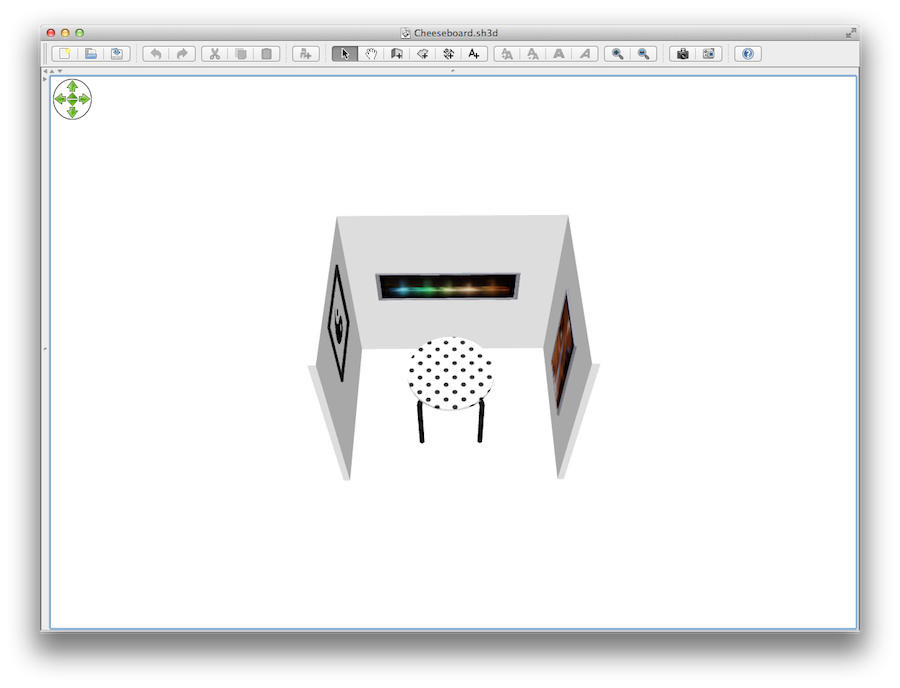
\includegraphics[scale=1]{Cheeseboard.png}
\caption{Layout of the Cheeseboard apparatus in the experimental space. The cheeseboard measured 1 m in diameter and was elevated 1 m from the floor.}
\label{fig:Cheeseboard}
\end{figure}

\textbf{Metric Processing}

Method:
Each mouse had previously been habituated to the clear and red experimental boxes. For the metric/coordinate test, two objects were placed in the box separated by 25 cm \(from inner edges\) and mice were allowed to explore the objects for 15 minutes. After a 5 min interval during which the mice were covered by a heavy cup, the objects were moved closer together to an 8 cm separation and the mouse was allowed to explore for 5 min. This procedure was carried out in the clear box that allowed the mouse to see the extra-maze, distal cues as well as in the red box that blocked the ability of the mouse to see these cues. Exploration during the last 5 min of habituation and during the 5 min test session were converted into a ratio value ranging [-1,1] to control for overall exploration. As such, a ratio value approaching -1 is interpreted as the mouse showing continued habituation and thus not noticing the change. A ratio value approaching 1 suggest the mouse dramatically explored the change.

\begin{figure}[h!]
\centering
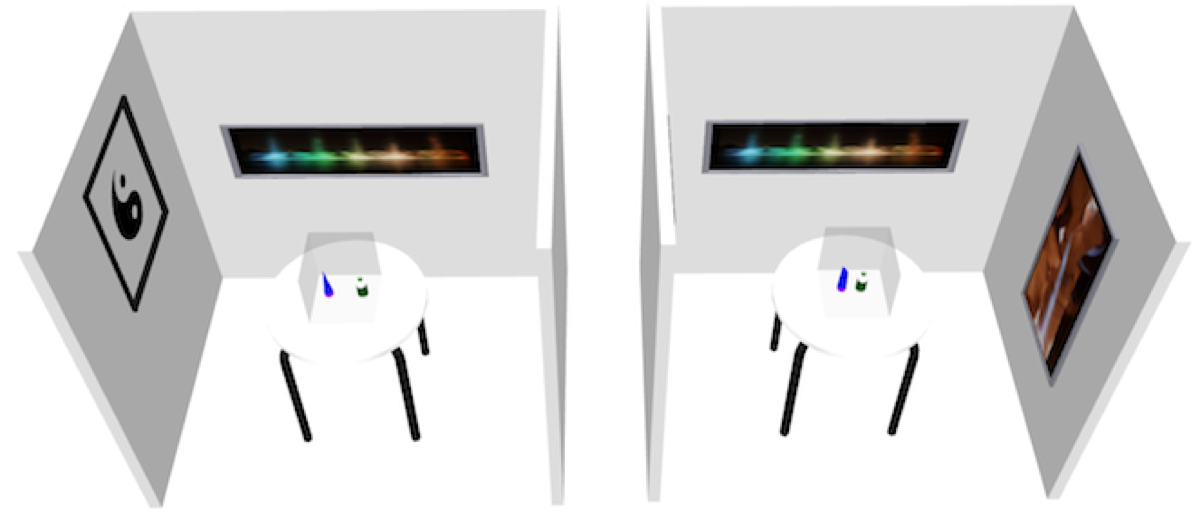
\includegraphics[scale=1]{Clear_Metric.png}
\caption{Layout of the Metric or Coordinate task in the experimental space. With the clear box, the mice were able to use distal cues to guide behavioral decisions}
\label{fig:Metric}
\end{figure}

\begin{figure}[h!]
\centering
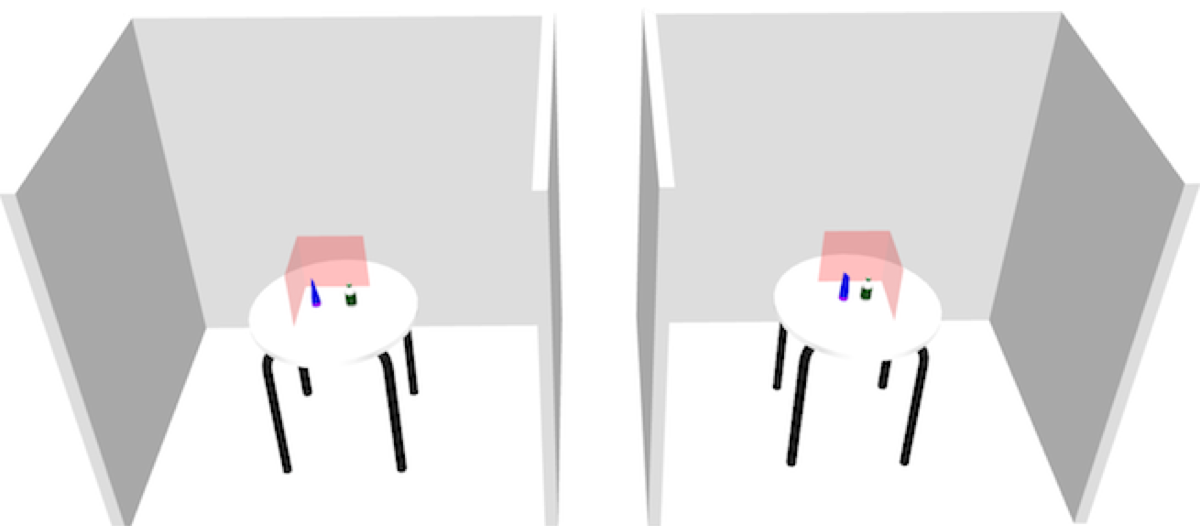
\includegraphics[scale=1]{Red_Metric.png}
\caption{Layout of the Metric or Coordinate task in the experimental space. With the red box, the mice did not have access to distal cues to guide behavioral decisions}
\label{fig:Metric}
\end{figure}

\textbf{Topological Processing}
Method:
Each mouse had previously been habituated to the clear and red experimental boxes. For the topological/categorical test, four objects were placed in a square in the box separated by 25 cm \(from inner edges\) and mice were allowed to explore the objects for 15 minutes. After a 5 min interval during which the mice were covered by a heavy cup, the front two objects were transposed, and the mouse was allowed to explore for 5 min. This procedure was carried out in the clear box that allowed the mouse to see the extra-maze, distal cues as well as in the red box that blocked the ability of the mouse to see these cues. Exploration during the last 5 min of habituation and during the 5 min test session were converted into a ratio value ranging [-1,1] to control for overall exploration. As such, a ratio value approaching -1 is interpreted as the mouse showing continued habituation and thus not noticing the change. A ratio value approaching 1 suggest the mouse dramatically explored the change.

\begin{figure}[h!]
\centering
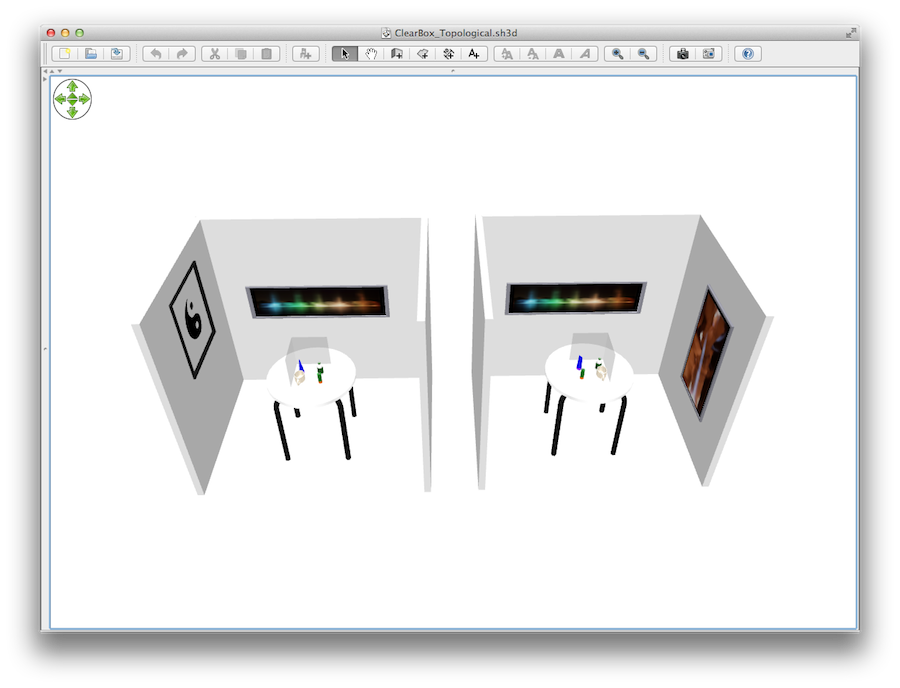
\includegraphics[scale=1]{Clear_Topological.png}
\caption{Layout of the Topological or Categorical task in the experimental space. With the clear box, the mice were able to use distal cues to guide behavioral decisions}
\label{fig:Topological}
\end{figure}

\begin{figure}[h!]
\centering
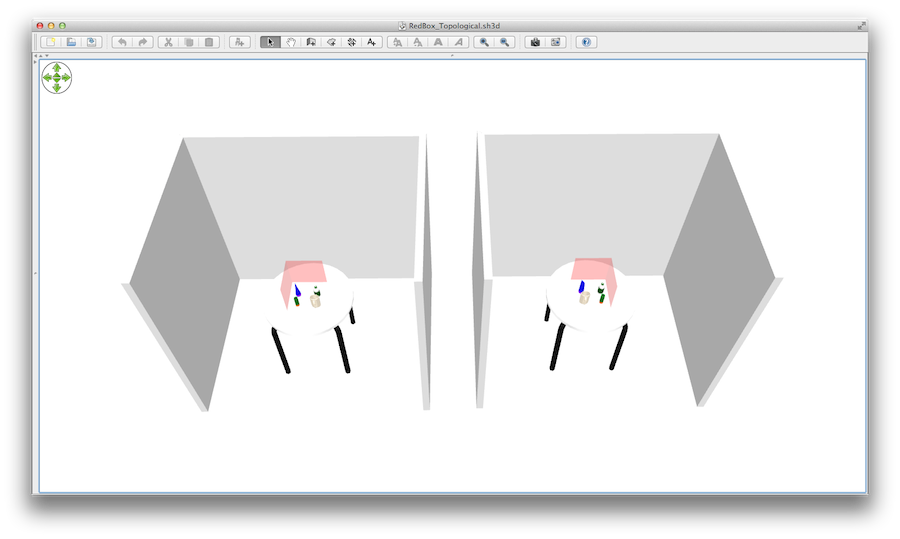
\includegraphics[scale=1]{Red_Topological.png}
\caption{Layout of the Topological or Categorical task in the experimental space. With the red box, the mice did not have access to distal cues to guide behavioral decisions}
\label{fig:Topological}
\end{figure}

\textbf{Location Recognition}

Method:
Each mouse had previously been habituated to the clear and red experimental boxes. For the location recognition test, two objects were placed in the box separated by 25 cm \(from inner edges\) and mice were allowed to explore the objects for 15 minutes. After a 5 min interval during which the mice were covered by a heavy cup, one of the objects was moved at a diagonal to a new location \(still 25 cm separation between the two objects\), and the mouse was allowed to explore for 5 min. This procedure was carried out in the clear box that allowed the mouse to see the extra-maze, distal cues as well as in the red box that blocked the ability of the mouse to see these cues. Exploration during the last 5 min of habituation and during the 5 min test session were converted into a ratio value ranging [-1,1] to control for overall exploration. As such, a ratio value approaching -1 is interpreted as the mouse showing continued habituation and thus not noticing the change. A ratio value approaching 1 suggest the mouse dramatically explored the change.

\begin{figure}[h!]
\centering
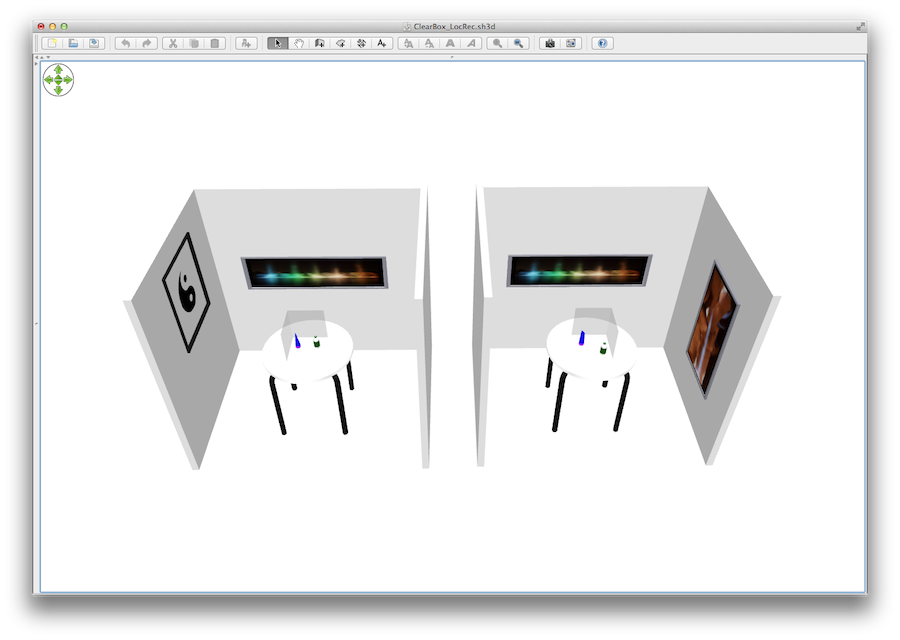
\includegraphics[scale=1]{Clear_LocationRecognition.png}
\caption{Layout of the Location Recognition task in the experimental space. With the clear box, the mice were able to use distal cues to guide behavioral decisions}
\label{fig:LocationRecognition}
\end{figure}

\begin{figure}[h!]
\centering
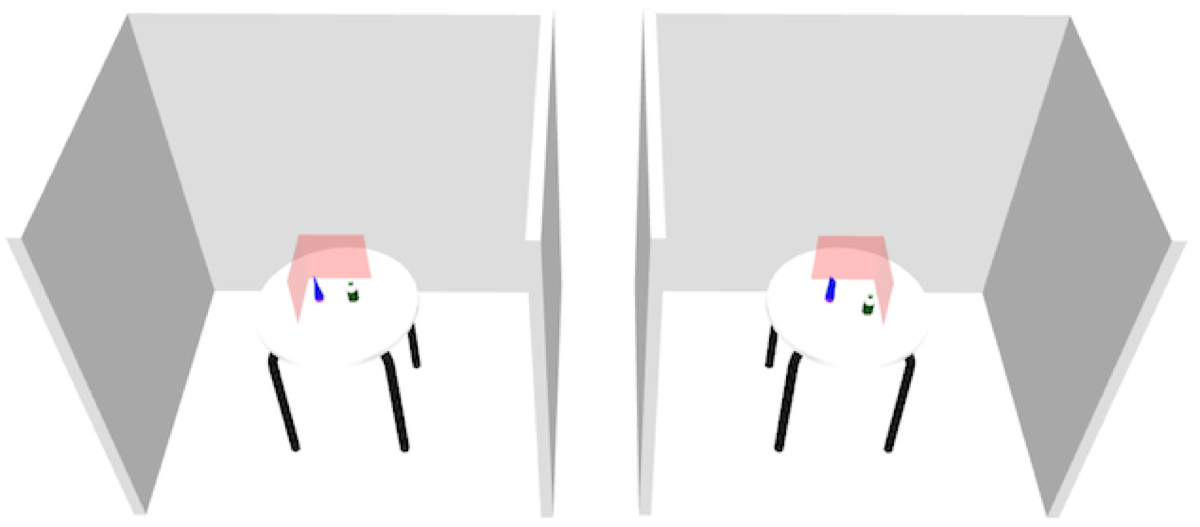
\includegraphics[scale=1]{Red_LocationRecognition.png}
\caption{Layout of the Location Recognition task in the experimental space. With the red box, the mice did not have access to distal cues to guide behavioral decisions}
\label{fig:LocationRecognition}
\end{figure}

\subsubsection{Temporal Attribute}
\textbf{Temporal Ordering for Visual Objects}

Method:
During session 1, two identical copies of a first object \(object 1\) were placed at the ends of the box 2.5 cm from the end walls and centered between the long walls. The mouse was placed in the center of the box facing away from both objects. The mouse was given 5 min to freely explore the objects. After 5 min, the mouse was removed to a small holding cup for 5 min. During this time, the first objects were replaced with two duplicates of a second object \(Object 2\). For Session 2, the mouse was again placed in the apparatus and allowed to explore. After 5 min, the mouse was removed to the holding cup for 5 min and the objects were replaced with two duplicates of a third object \(Object 3\). For Session 3, the mouse was given 5 min to explore. After 5 min, the mouse was removed into a small cup for 5 min and an unused copy of the first and an unused copy of the third object were placed into the box. The mouse was again placed into the box and allowed to explore the two objects \(i.e., Objects 1 and 3\) during a 5 min test session. This procedure was carried out in the clear box that allowed the mouse to see the extra-maze, distal cues as well as in the red box that blocked the ability of the mouse to see these cues. Exploration of each object during the test session were converted into a ratio value ranging [-1,1] to control for overall exploration. As such, a ratio value approaching -1 is interpreted as the mouse showing an absolute preference for the third over the first object. A ratio value approaching 1 suggest the mouse strongly explored the first over the third object.

\begin{figure}[h!]
\centering
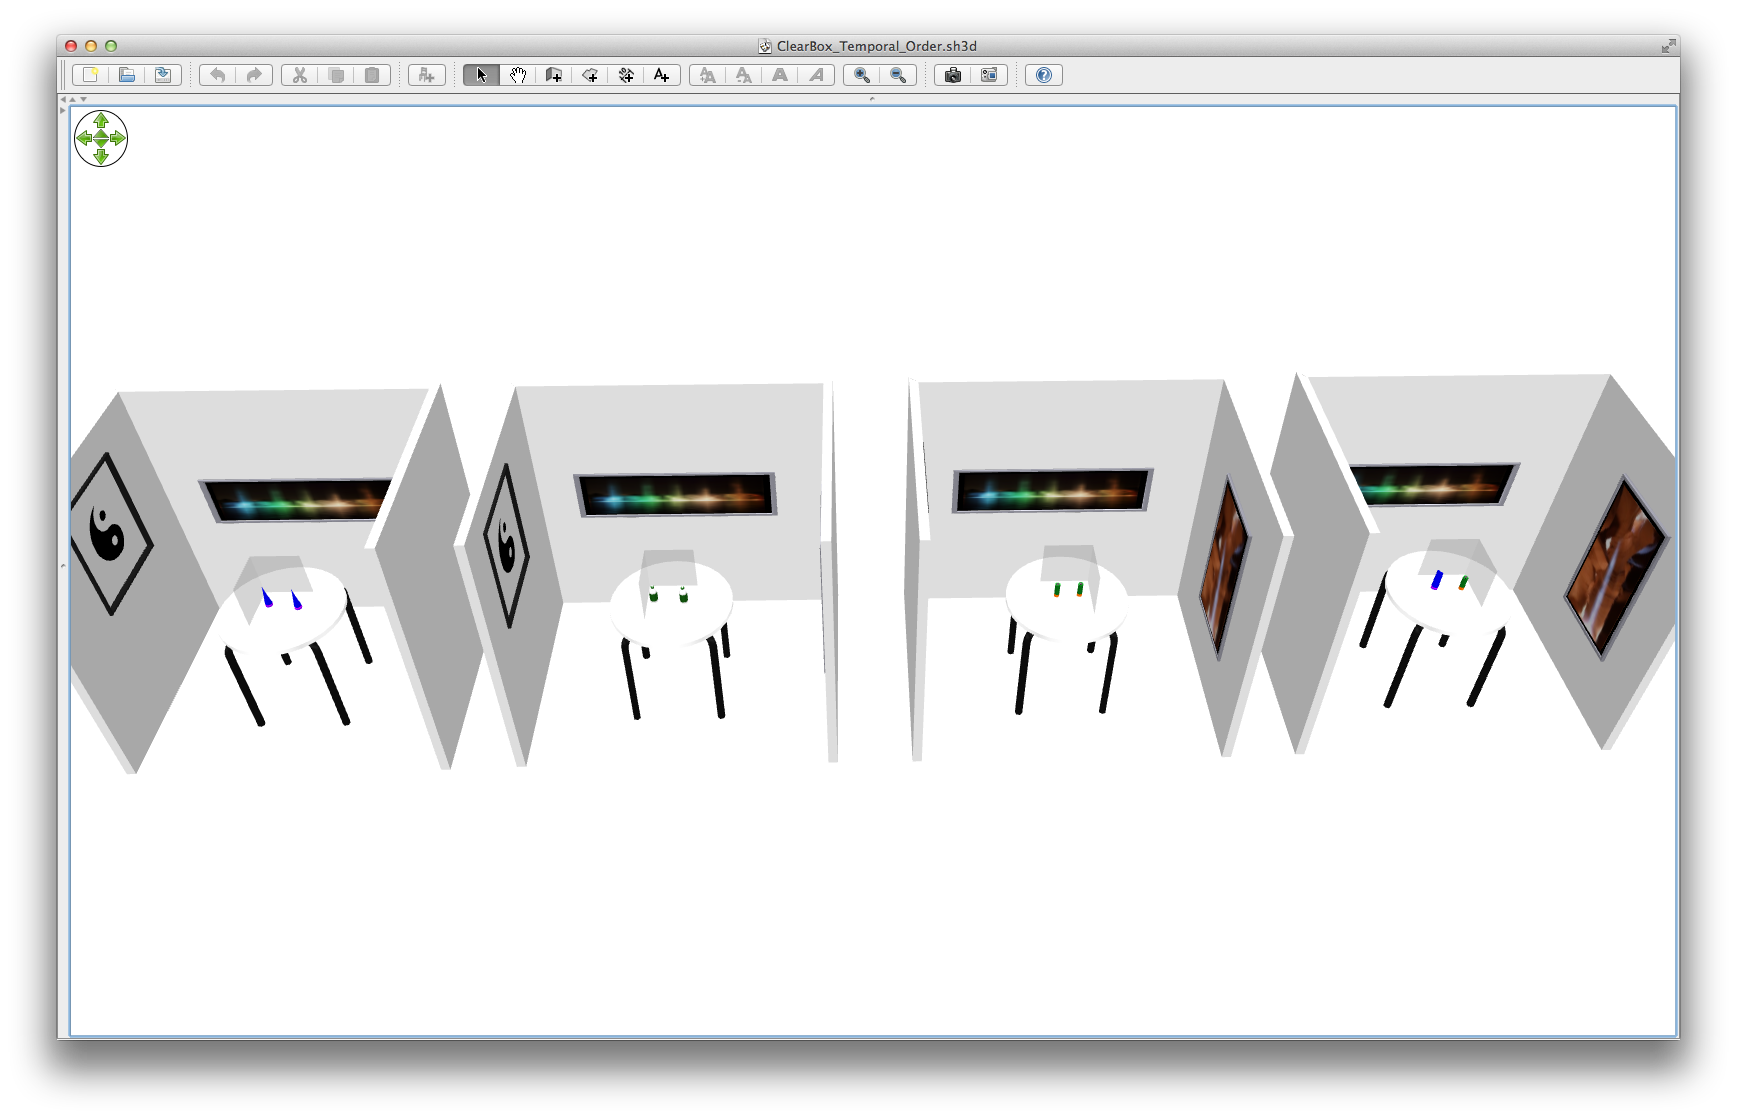
\includegraphics[scale=1]{Clear_TemporalOrdering.png}
\caption{Layout of the Temporal Ordering for Visual Objects task in the experimental space. With the clear box, the mice were able to use distal cues to guide behavioral decisions}
\label{fig:Temporal Ordering}
\end{figure}

\begin{figure}[h!]
\centering
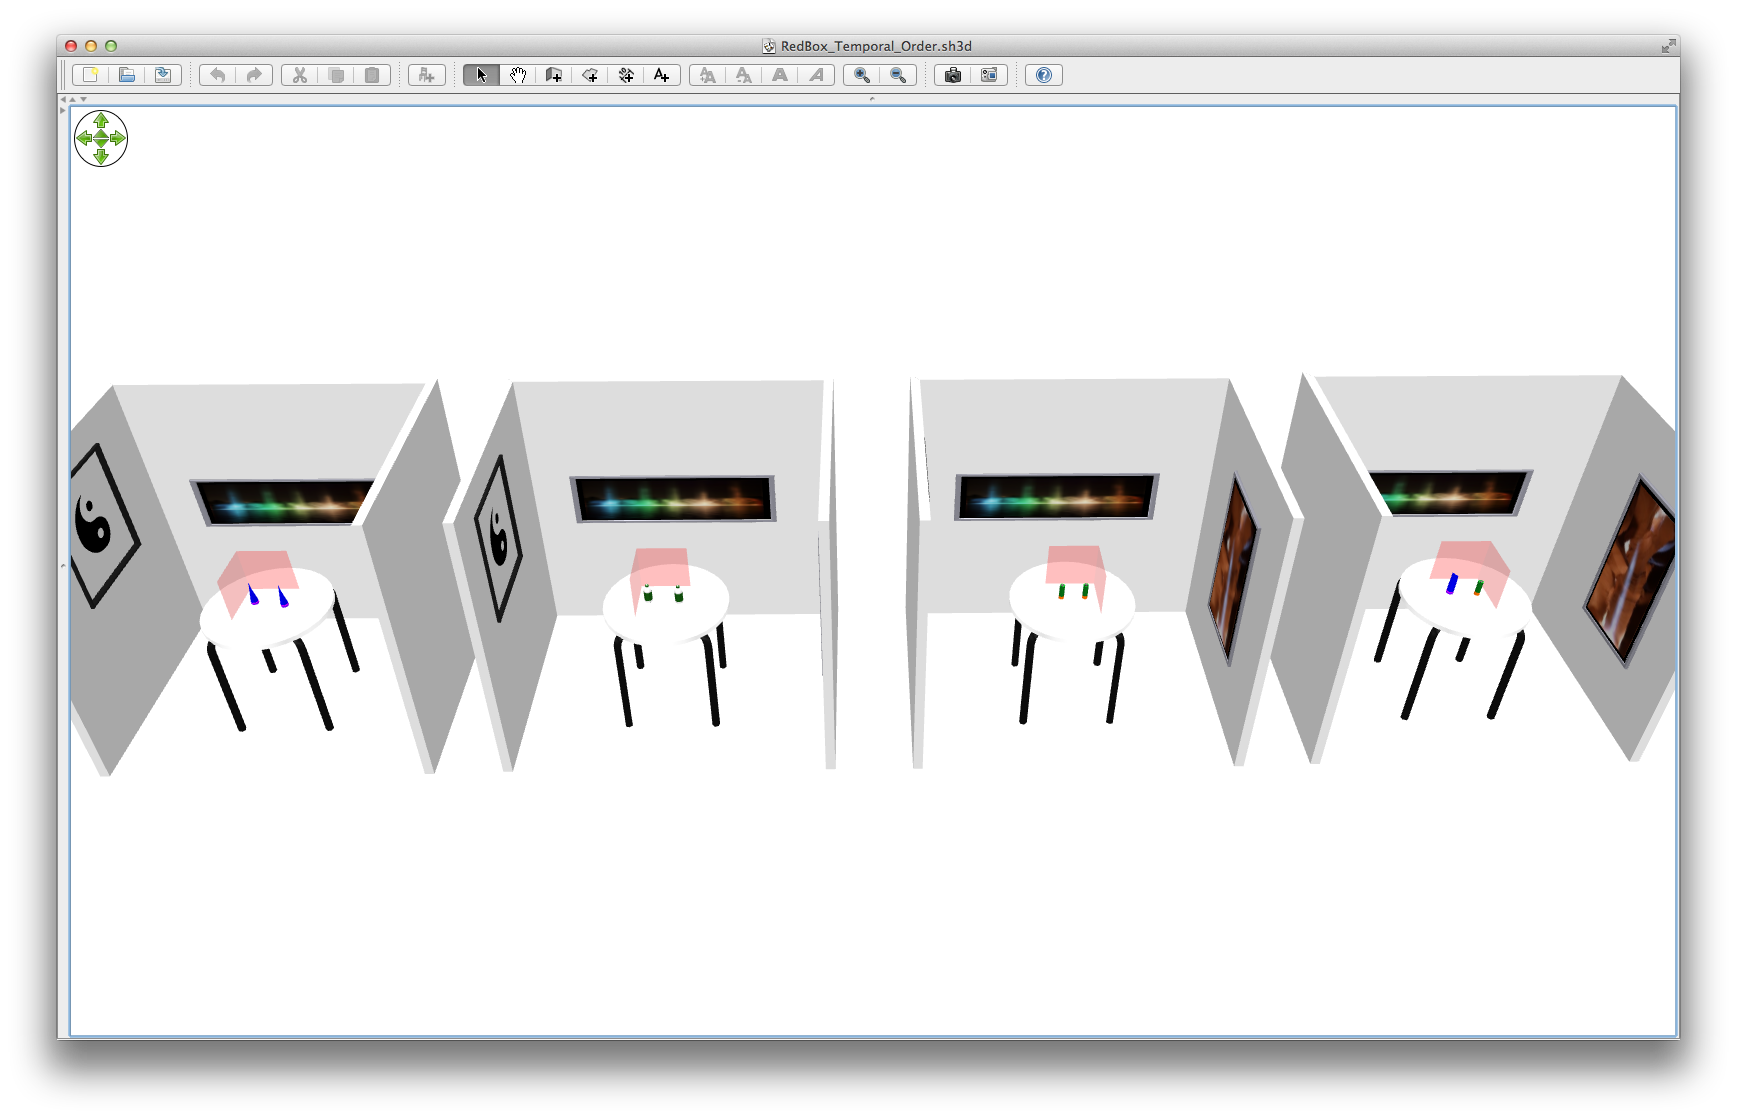
\includegraphics[scale=1]{Red_TemporalOrdering.png}
\caption{Layout of the Temporal ordering for Visual Objects task in the experimental space. With the red box, the mice did not have access to distal cues to guide behavioral decisions}
\label{fig:Temporal Ordering}
\end{figure}

\textbf{Temporal Order Control: Novelty Detection for Visual Objects}

Method:
In addition to reflecting impaired temporal ordering, increased exploration of the first object over the third could also be interpreted as being due to difficulty in remembering the first object prior to the test session. To minimize and con- trol for such general memory deficits, a novelty detection of visual objects task was performed. Briefly, on a different day mice received three sessions during which they were allowed to explore three novel sets of objects \(Objects 4, 5, 6\) similarly to the temporal ordering tasks. During the test session, the first object and a novel fourth object \(Object 7\) were presented and the mice were allowed 5 min to explore. This procedure was carried out in the clear box that allowed the mouse to see the extra-maze, distal cues as well as in the red box that blocked the ability of the mouse to see these cues. Exploration of each object during the test session were converted into a ratio value ranging [-1,1] to control for overall exploration. As such, a ratio value approaching -1 is interpreted as the mouse showing an absolute preference for the familiar over the novel object. A ratio value approaching 1 suggest the mouse strongly explored the novel over the familiar object.

\begin{figure}[h!]
\centering
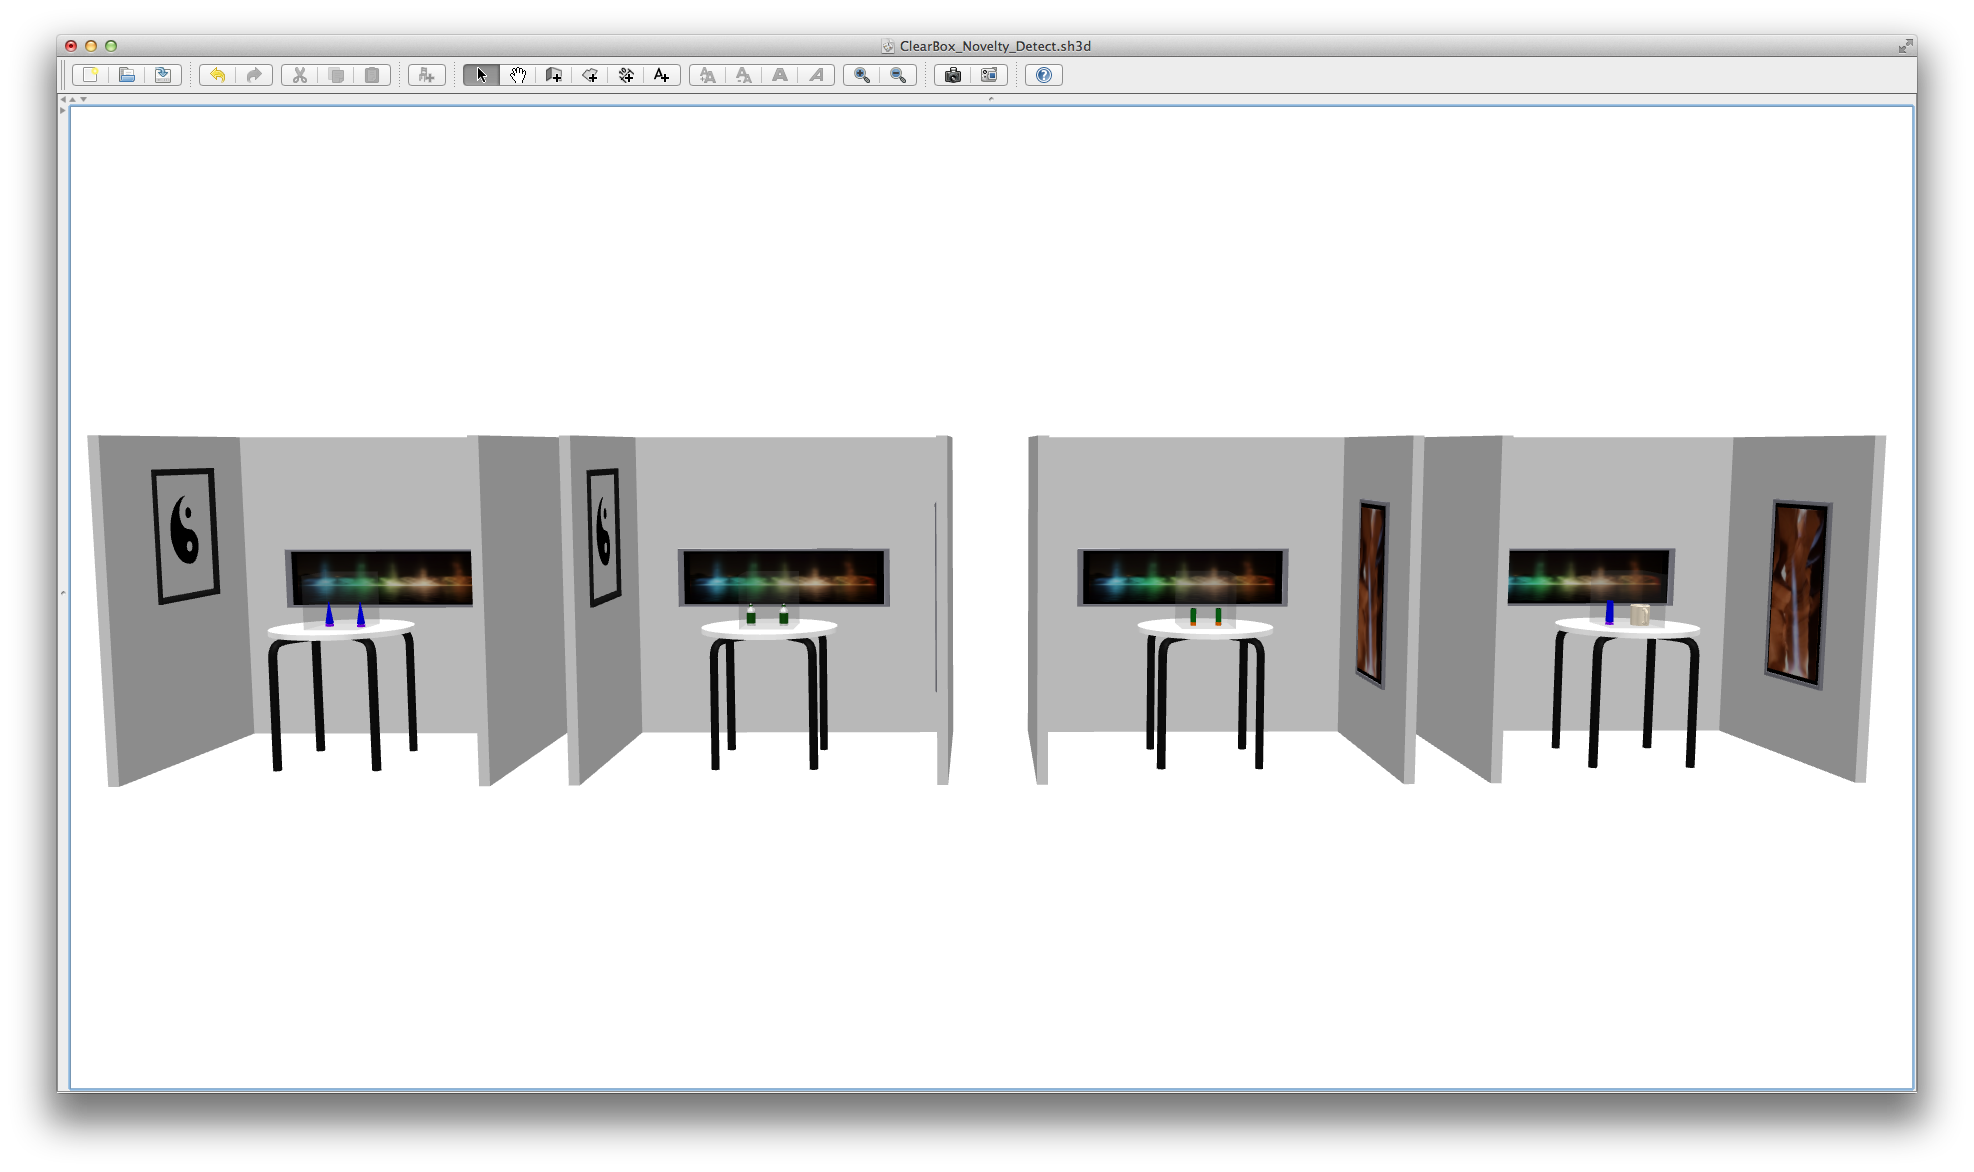
\includegraphics[scale=1]{Clear_NoveltyDetection.png}
\caption{Layout of the Novelty Detection for Visual Objects task in the experimental space. With the clear box, the mice were able to use distal cues to guide behavioral decisions}
\label{fig:Novelty Detection}
\end{figure}

\begin{figure}[h!]
\centering
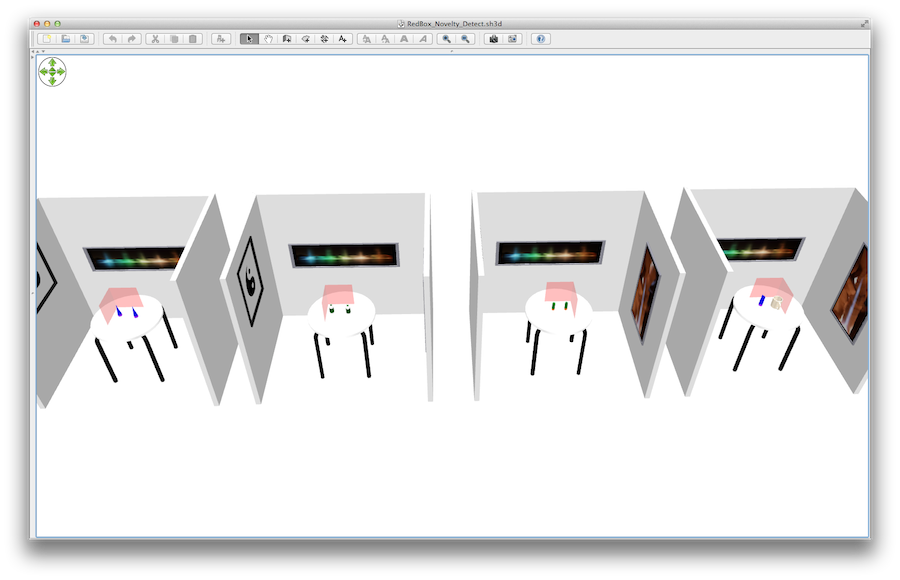
\includegraphics[scale=1]{Red_NoveltyDetection.png}
\caption{Layout of theNovelty Detection for Visual Objects task in the experimental space. With the red box, the mice did not have access to distal cues to guide behavioral decisions}
\label{fig:Novelty Detection}
\end{figure}

\subsubsection{Sensory/Perceptual Attributes}
\textbf{Feature Ambiguity}

Method:
Each mouse had previously been habituated to the clear and red experimental boxes. For the configural recognition condition, mice were placed for 15 min in the red box containing two compound objects, AB and CD, separated by 15 cm. Following a 5 min delay under a heavy cup, the mouse underwent a 5-min Test Phase in which one object from the Study Phase remained the same \(AB\) and the other compound object is created from one component of each of the previous familiar objects, \(e.g., AD\). That is, the “novel” object \(AD\) is composed of the same elements, but rearranged into a novel configuration. Therefore, the object is “novel” by virtue of its configuration, not by its elements, each of which was present in one of the original compound stimuli. Exploration of each compound object was scored as a single unit. Exploration during the last 5 min of habituation and during the 5 min test session were converted into a ratio value ranging [-1,1] to control for overall exploration. As such, a ratio value approaching -1 is interpreted as the mouse showing continued habituation and thus not noticing the change. A ratio value approaching 1 suggest the mouse dramatically explored the change.


\begin{figure}[h!]
\centering
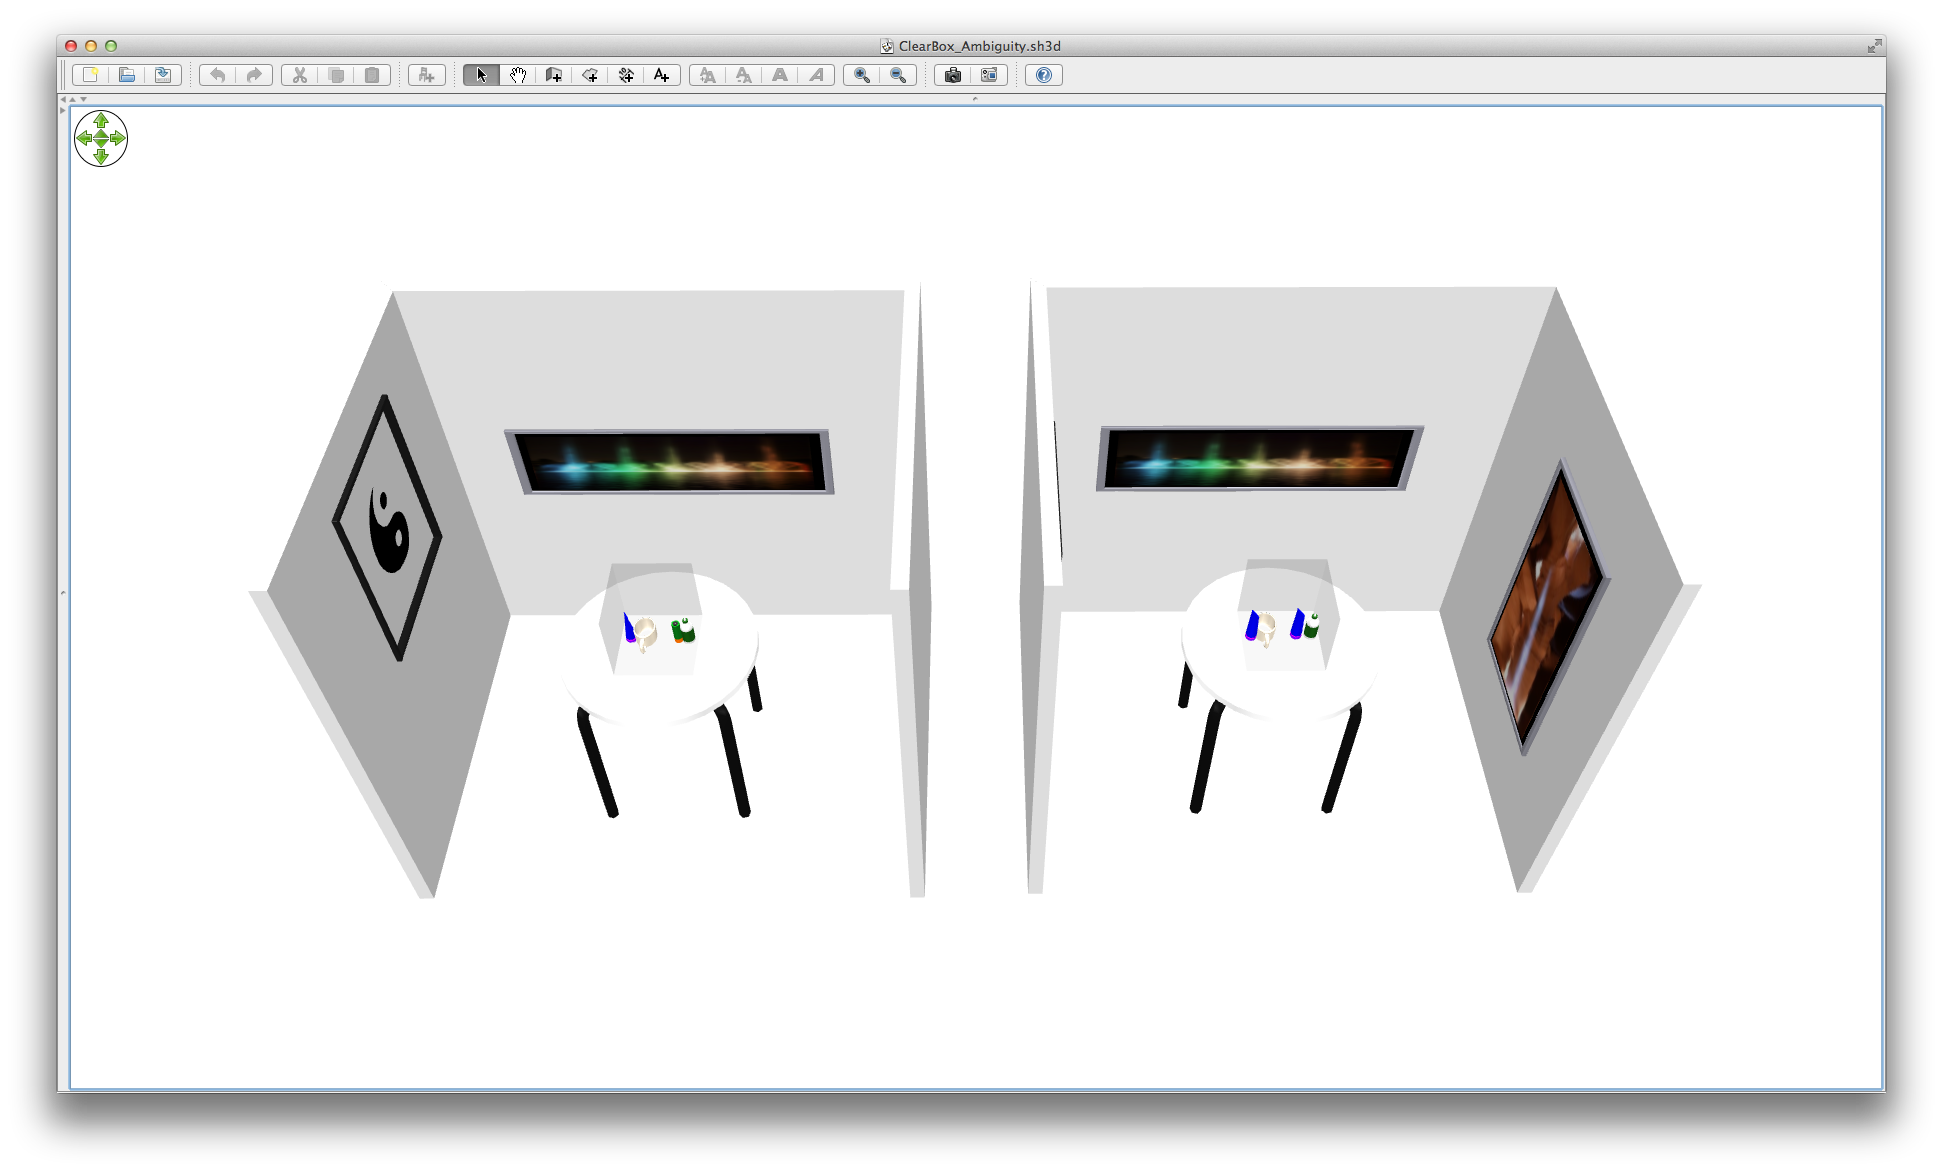
\includegraphics[scale=1]{Clear_Ambiguity.png}
\caption{Layout of the Configural Ambiguity task in the experimental space. With the clear box, the mice were able to use distal cues to guide behavioral decisions}
\label{fig:Ambiguity}
\end{figure}

\begin{figure}[h!]
\centering
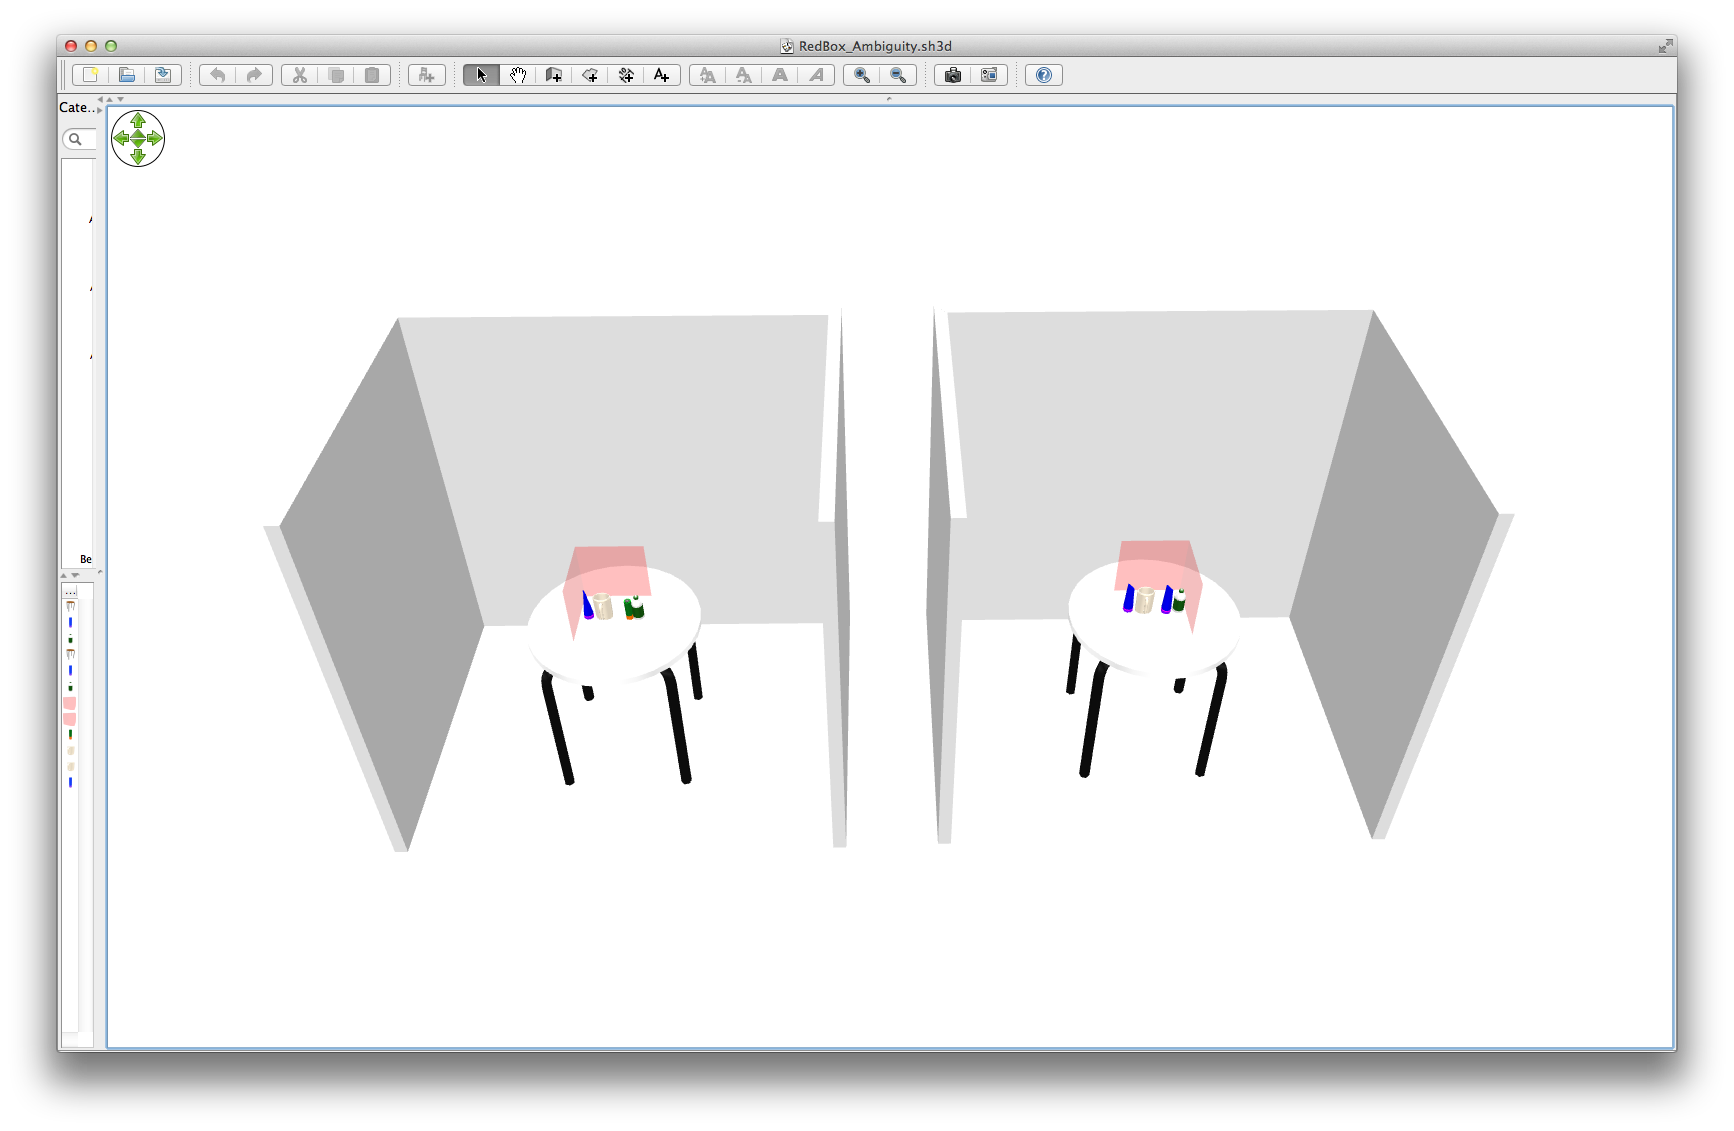
\includegraphics[scale=1]{Red_Ambiguity.png}
\caption{Layout of the Configural Ambiguity task in the experimental space. With the red box, the mice did not have access to distal cues to guide behavioral decisions}
\label{fig:Ambiguity}
\end{figure}


\textbf{Feature Ambiguity Control: Novelty Detection for Configural Objects}

Method:
Each mouse had previously been habituated to the clear and red experimental boxes. For the configural recognition condition, mice were placed for 15 min in the red box containing two compound objects, AB and CD, separated by 15 cm. Following a 5 min delay under a heavy cup, the mouse underwent a 5-min control task during which CD was replaced by two never before seen objects \(EF\) was also performed. This procedure was carried out in the clear box that allowed the mouse to see the extra-maze, distal cues as well as in the red box that blocked the ability of the mouse to see these cues. Exploration during the last 5 min of habituation and during the 5 min test session were converted into a ratio value ranging [-1,1] to control for overall exploration. As such, a ratio value approaching -1 is interpreted as the mouse showing continued habituation and thus not noticing the change. A ratio value approaching 1 suggest the mouse dramatically explored the change.

\begin{figure}[h!]
\centering
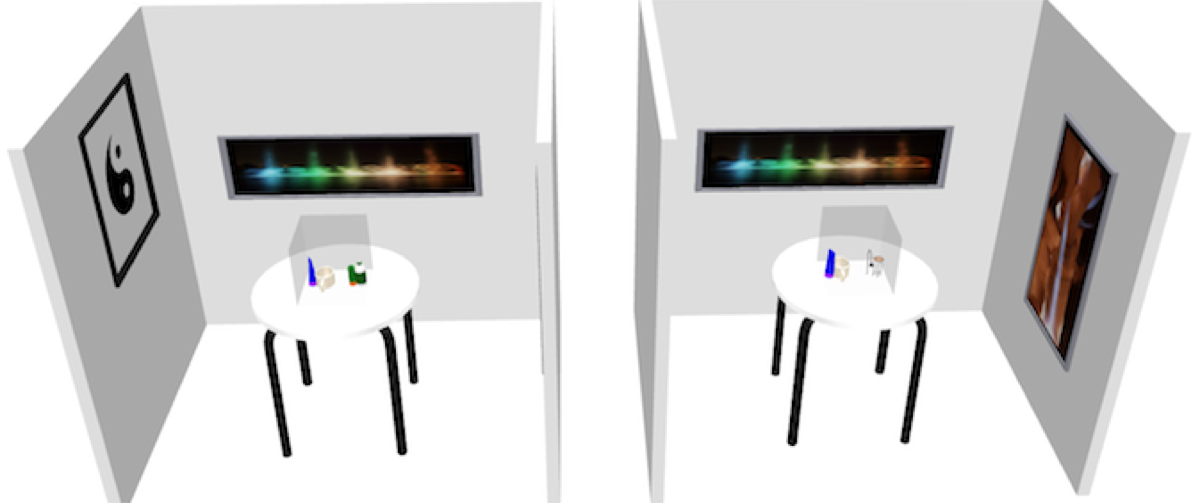
\includegraphics[scale=1]{Clear_Ambiguity_Control.png}
\caption{Layout of the Configural Ambiguity Control task in the experimental space. With the clear box, the mice were able to use distal cues to guide behavioral decisions}
\label{fig:Ambiguity Control}
\end{figure}

\begin{figure}[h!]
\centering
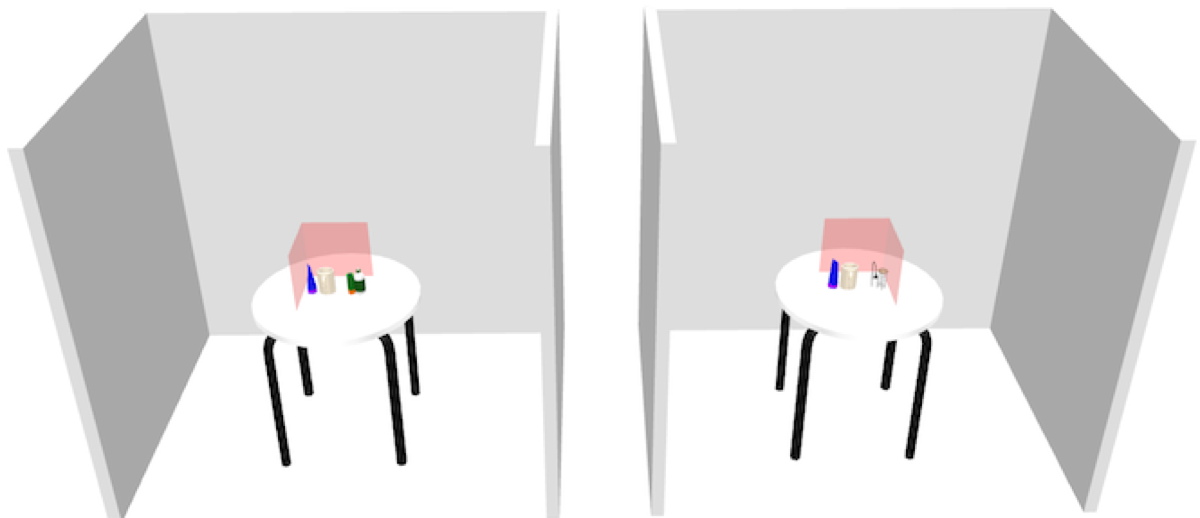
\includegraphics[scale=1]{Red_Ambiguity_Control.png}
\caption{Layout of the Configural Ambiguity Control task in the experimental space. With the red box, the mice did not have access to distal cues to guide behavioral decisions}
\label{fig:Ambiguity Control}
\end{figure}

\textbf{Object Recognition at 1 hour and 24 hour delays}

Method:
Each mouse had previously been habituated to the clear and red experimental boxes. For the object recognition test, two objects were placed in the box separated by 25 cm \(from inner edges\) and mice were allowed to explore the objects for 15 minutes. After a 5 min interval during which the mice were covered by a heavy cup, one of the objects was replaced by a novel object that had never before been experienced byt he mouse, and the mouse was allowed to explore for 5 min. This procedure was carried out in the clear box that allowed the mouse to see the extra-maze, distal cues as well as in the red box that blocked the ability of the mouse to see these cues. This procedure was carried out in each box separately for delays of 1 hour and 24 hours. Exploration during the last 5 min of habituation and during the 5 min test session were converted into a ratio value ranging [-1,1] to control for overall exploration. As such, a ratio value approaching -1 is interpreted as the mouse showing continued habituation and thus not noticing the change. a ratio value approaching 1 suggest the mouse dramatically explored the change.

Layout of the Configural Ambiguity Control task in the experimental space. With the red box, the mice did not have access to distal cues to guide behavioral decisions

\begin{figure}[h!]
\centering
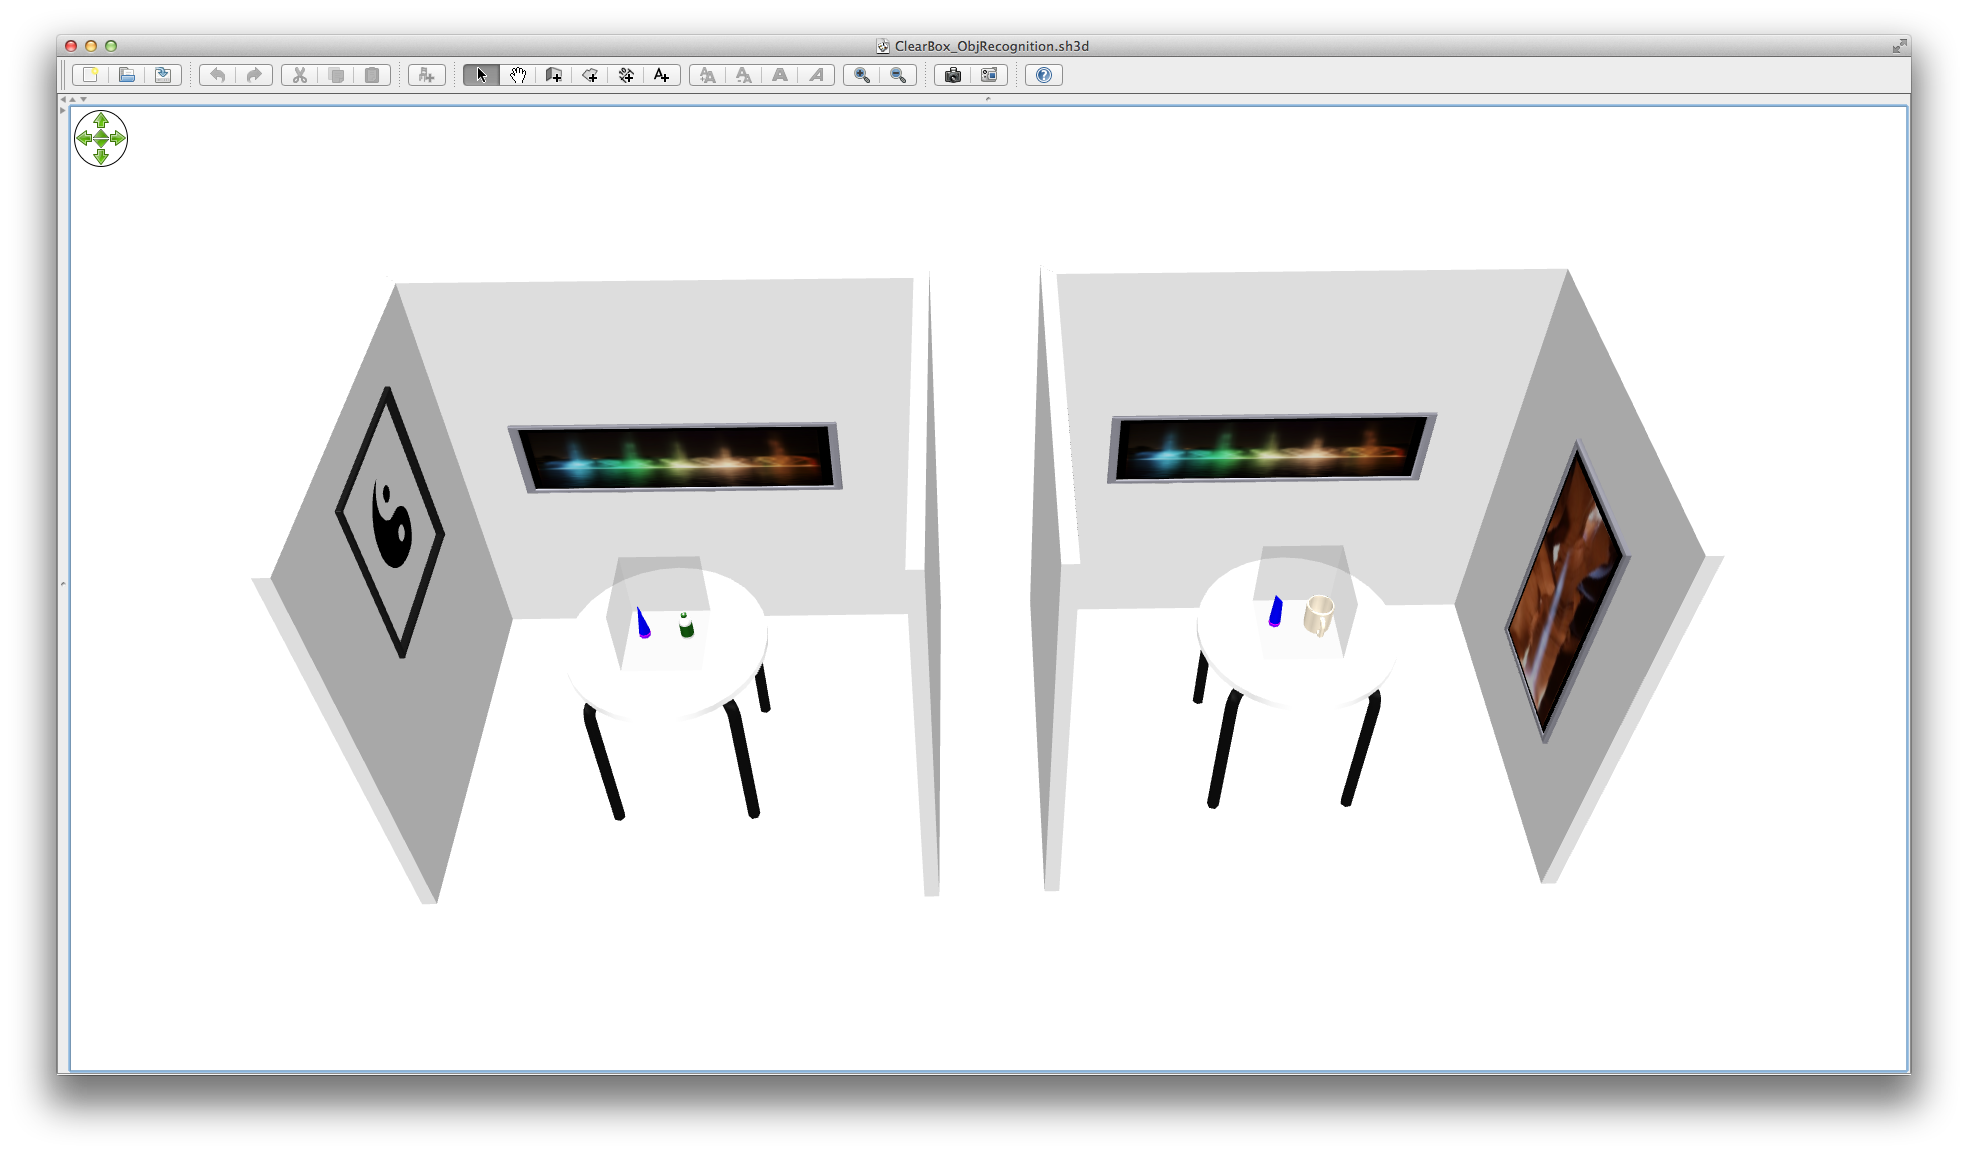
\includegraphics[scale=1]{Clear_ObjectRecognition.png}
\caption{Layout of the Object Recognition task in the experimental space. With the clear box, the mice were able to use distal cues to guide behavioral decisions}
\label{fig:Ambiguity Control}
\end{figure}

\begin{figure}[h!]
\centering
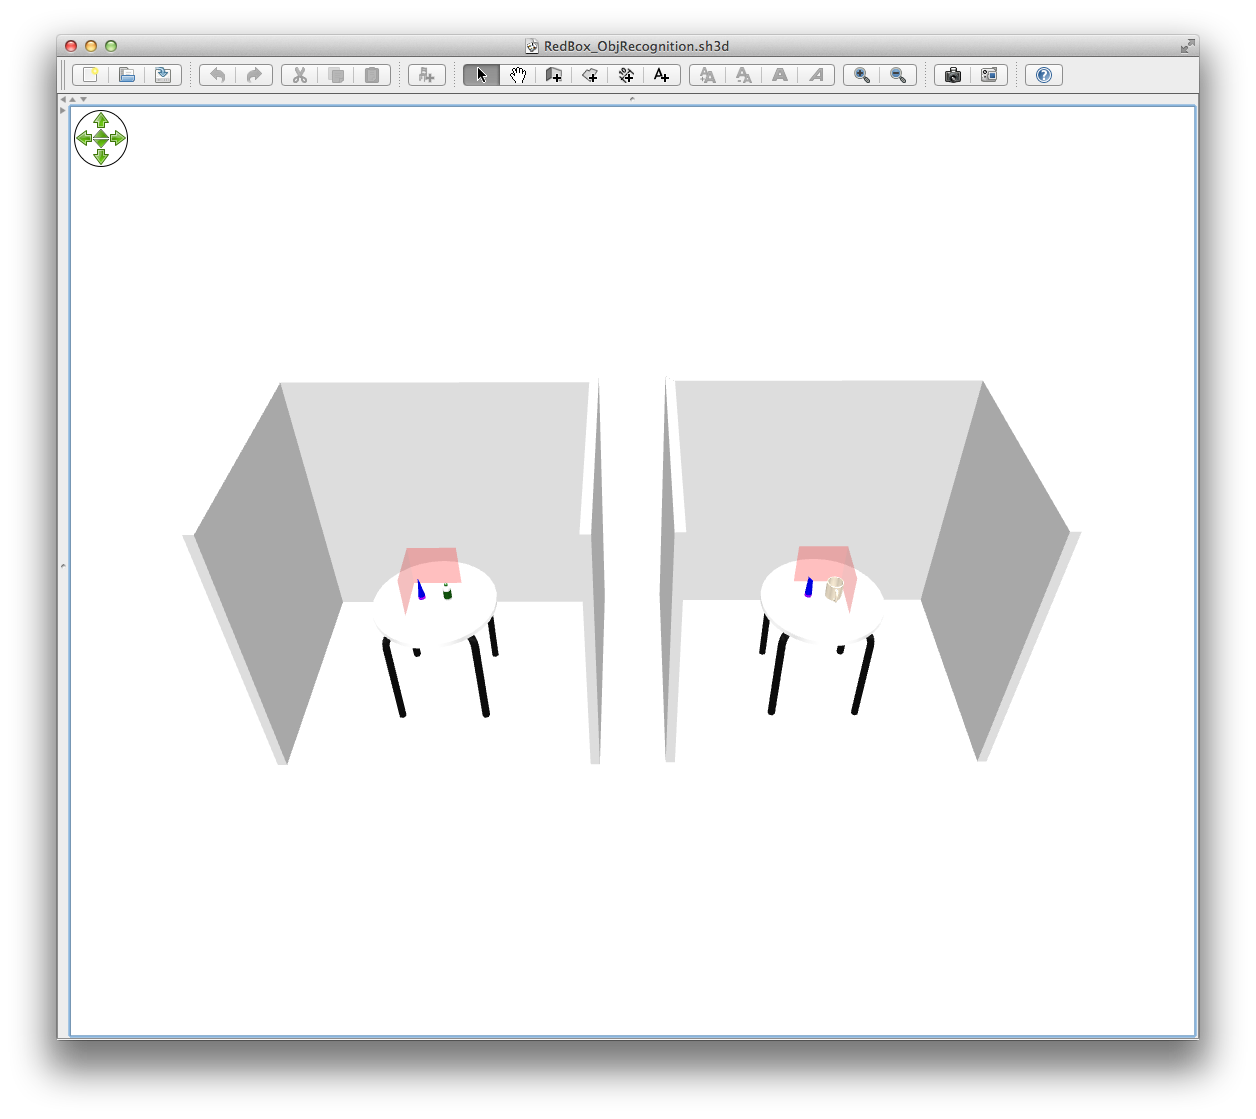
\includegraphics[scale=1]{Red_ObjectRecognition.png}
\caption{Layout of the Object Recognition task in the experimental space. With the red box, the mice did not have access to distal cues to guide behavioral decisions}
\label{fig:Ambiguity Control}
\end{figure}

\subsubsection{Tests of Executive Function}
\textbf{Spontaneous Alternation}

Method:
Mice were placed in the stem of a Y maze and allowed to explore. Whenever the mouse entered one of the arms of the Y maze with all four limbs their response was recorded. Upon reaching the end of the arm, the mouse was gently picked up and replaced in the stem of the Y maze. The number of times the mouse alternated \(i.e., did not repeat the previous turn\), it was recorded as an alternation.

\textbf{Response Learning}

Method:
Mice were placed in the stem of a plus maze with one of the arms blocked off \(forming a T maze\). Mice were given five trials to determine if there was any preference for one direction over the other. As no such preference was observed, mice were randomly assigned the rule to turn right or turn left. Mice received 20 trials per day for 4 days. Entry into an arm with all four limbs was recorded as a choice and mice were not allowed to self correct when they made mistakes. Upon reaching the end of the arm, the mouse was gently picked up and replaced in the stem of the plus maze.

\textbf{Reversal Learning}

Method:
The day after mice finished training on response learning, they received 80 trials of reversal training. This means that the turn the mice had just learned to make for reward was now incorrect, rather the mice had to make the opposite turn to receive reward. Upon reaching the end of the arm, the mouse was gently picked up and replaced in the stem of the plus maze. Number of previously correct choices made were recorded as errors and error type was evaluated as perseverative or regressive based on the work of Aggleton and Ragozzino. Additionally, a behavioral change point algorithm was used to define the point at which each mouse consistently switched their responses from the previously learned rule to the new rule.

\subsubsection{Motor Function}
\textbf{Capellini Handling}

Method:
Mice were habituated over a weekend to dried capellini pasts in their cages. Each mouse was placed in a 250 mL beaker and given a 5 cm piece of dried capellini. Their behaviors while eating were recorded for an offline analysis of their motor behaviors. Their latency to finish each piece of pasta was recorded, as were abnormal behaviors including the mouse having its paws together while eating, losing contact with the pasta with one or both paws, and using the mouth to pull the pasta rather than using the digits to feed the pasta into the mouth.

\textbf{Parallel Rung Walking}

Method:
Mice were placed in a box measuring 15 cm squared with 1.5 mm diameter parallel rungs making up the floor. The mice were allowed to freely explore the box for 5 minutes. The number of times a paw slipped through the parallel rod floor beyond the wrist or ankle, a "foot slip" error was recorded. The total number of steps were also recorded to use as a normalizing factor.

\subsubsection{Adaptive Function}
\textbf{Nesting Behaviors}

Method:
Sawdust was used to fill a 10 cm long piece of 2" \(~5 cm\) diameter PVC pipe that was capped at one end. This pipe was placed in a cage with each mouse and the latency to contact the sawdust in the pipe, the latency to start digging in the sawdust, and the latency to finalize the nest were recorded.

\textbf{Neophobia}

Method:
Mice were given three neophobia tests. The first was in their homecage. Each mouse was provided a food they had never encountered \(Cheerios cereal\) and the latcny to take the first bite was recorded. The second test was each mouse was placed on a large platter in a bright area int he testing room and the latency to take a bite from a reward pellet \(familiar food\) was recorded. The final test consisted of each mouse being placed in a novel white box and fed a Cheerio that had been stored with thyme overnight, resulting in a novel food. Again, latency to take the first bite was recorded.

\subsection{Statistical Analysis}
\subsubsection{Dependent Measures and Data Visualization.}

For exploratory tasks, ratio values were computed after the following formula: Exploration of the object of interest \(or all objects in the 5 min session of interest\) minus the exploration of the other objects or last 5 min of the habituation session. This was divided by the sum of all exploration across both sessions or of both objects. As a formula this is depicted as: \(A-B\)/\(A+B\).

For the reversal learning, the number of perseverative errors \(continuing old rule\) during the first 20 \(1-20\) trials were computed. The number of regressive errors \(returning to old rule\) were calculated during trials 21-40. A frequentist change point algorithm developed by Gallistel and colleagues \(2004\) was used to compute the point at which each mouse showed evidence for having learned to apply the new rule.

Data are all plotted in DataGraph \(3.21 beta, Visual Data Tools, Inc. Chapel Hill, NC.\). Ratio data and computed factors are plotted as a bar plot to the mean with all collected data points overlain. Repeated data are presented as a line graph at the mean of each block, with all data points overlain.

\subsubsection{Tests for equal variance and heteroscedasticity.}

Prior to statistical analyses, the data were tested for normalcy \(Shapiro Wilk test\) and homoscedacity \(Browne Forsythe test\). Repeated measures were evaluated for sphericity using Mauchly's test of sphericity using R 3.0.1.

\subsubsection{Parametric Statistical Analysis}

Once deemed appropriate, further statistical analyses were performed using parametric analyses of variance. For exploratory task ratios and computed factors were compared using a one-way analysis of variance \(ANOVA\) with groups \(2N control, Ts65Dn\). For acquisition tasks wherein learning was quantified across trials as well as locomotor data, statistical analyses were performed using a mixed model ANOVA with group \(2N control, Ts65Dn\) as a between groups factor and block of trials as a repeated within factor. If locomotor activity was significantly different between the groups, locomotor activity was included in the statistical analysis as a covariate.

All results were considered significant at an alpha < .05 and Power \(1-beta\) > .8: Analyses were performed to determine observed power and effect size for all reported effects. Statistical analyses were performed in R 3.0.1. language and environment and statistical power was calculated using both R and the statistical program GPower 3. All reported p values were adjusted for False Discovery Rate using a custom script written in R 3.0.1.

\subsubsection{Principal Component Analyses}

PCA were run by applying the functions in the FactoMineR package in R 3.0.1 and follow up analyses with functions in the MClust, HClust, PVClust, and Psych packages. These models are presented to provide a qualitative description of the experiments tasks and to demonstrate that the behavioral domain evaluated by these tasks parallel the cognitive domains studied using the ACTB in populations with with Down Syndrome.


\section{Results}
\subsection{Spatiotemporal Processing}
\subsubsection{Spatial Attribute}

textbf{Cheeseboard}

\begin{figure}[h!]
\centering
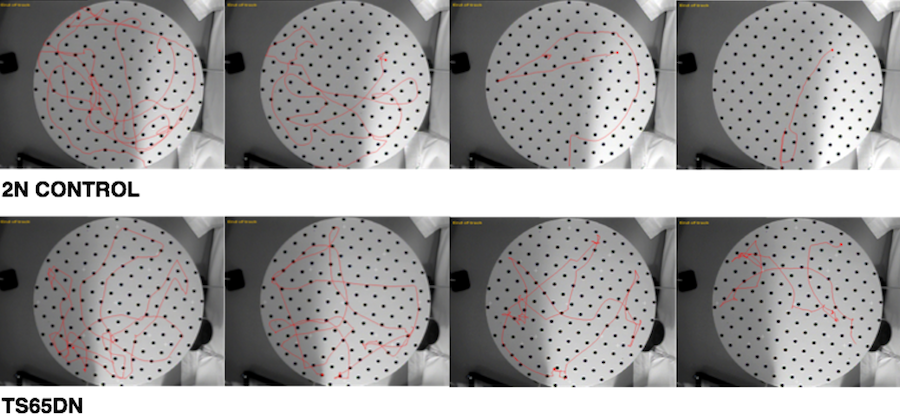
\includegraphics[scale=1]{Cheeseboard_TRACK.png}
\caption{Top. 2N wildtype mouse performance on cheeseboard. Bottom. Ts65Dn mouse performance on cheeseboard}
\label{fig:Cheeseboard Track}
\end{figure}

For unadjusted raw latency, Ts65Dn mice took significantly longer to find the reward than 2N control mice. There was a main effect for groups (F(1,76)=185.645,p<2e-16), a main effect for block of trials (F(1,76)=663.876,p<2e-16). There was no interaction among group and block (F(1,76)=0.333,p=.566).

When one scaled the latency data to account for differential performance during block 1, a different pattern of data emerge. There is still an effect for groups (F(1,76)=48.44,p=1.05e-9) as well as an effect for blocks (F(1,76)=766.64,p<2e-16). However, when the data are scaled for performance on block 1, a clear interaction emerges wherein the Ts65Dn mice show a more shallow learning curve than 2N control mice (F(1,76)=14.74,p=.000253).

\begin{figure}[h!]
\centering
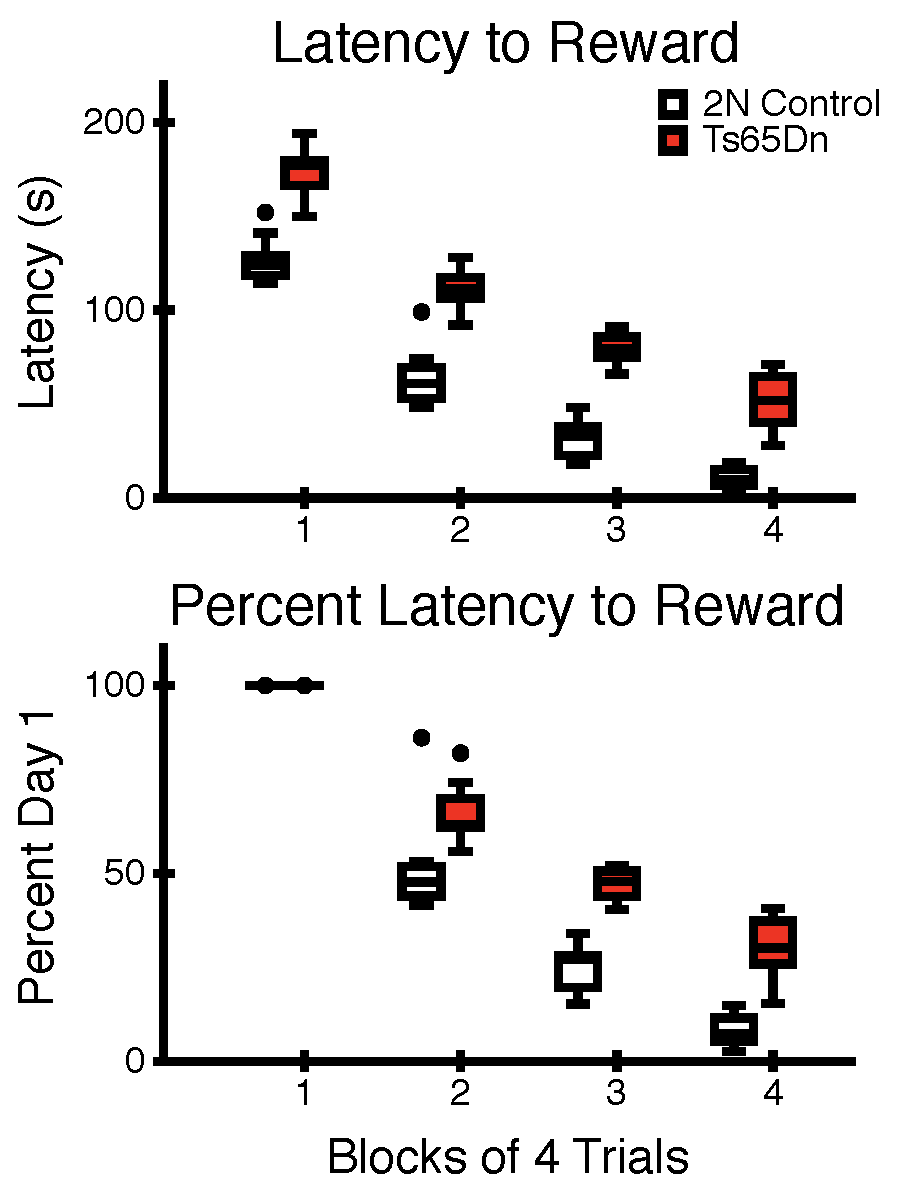
\includegraphics[scale=1]{Cheeseboard_Latency.pdf}
\caption{Top. Raw latency (s) to obtain reward. Bottom. Percent latency to obtain reward each day scaled by latency on Day 1}
\label{fig:Cheeseboard Latency}
\end{figure}

For unadjusted raw distance, Ts65Dn mice took significantly longer to find the reward than 2N control mice. There was a main effect for groups (F(1,76)=88.406,p<2.27e-14), a main effect for block of trials (F(1,76)=149.318,p<2e-16). There was no interaction among group and block (F(1,76)=0.258,p=.613).

When one scaled the distance data to account for differential performance during block 1, a different pattern of data emerge. There is still an effect for groups (F(1,76)=25.194,p=3.32e-6) as well as an effect for blocks (F(1,76)=137.217,p<2e-16). However, when the data are scaled for performance on block 1, a trend toward a significant interaction emerges wherein the Ts65Dn mice show a more shallow learning curve than 2N control mice (F(1,76)=3.887,p=.0523).

\begin{figure}[h!]
\centering
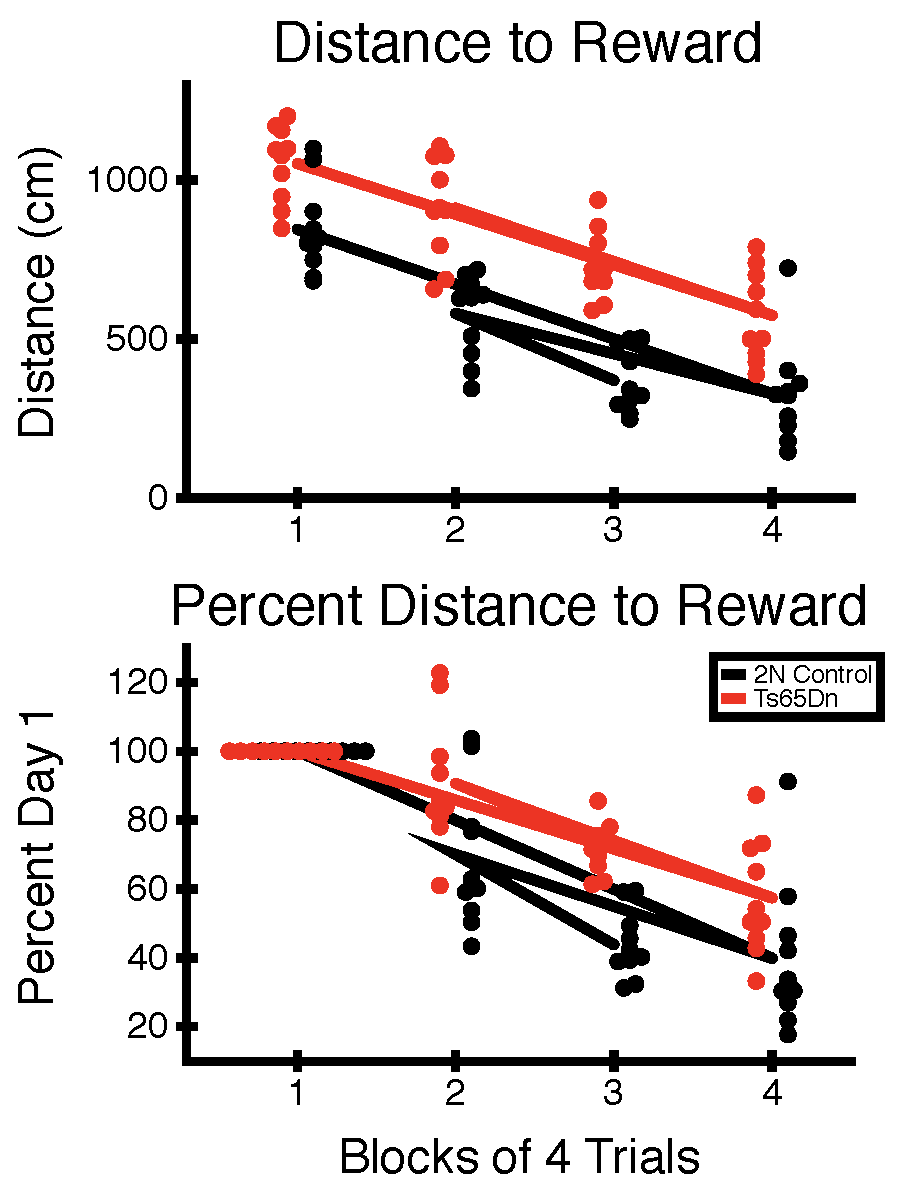
\includegraphics[scale=1]{Cheeseboard_Distance.pdf}
\caption{Top. Raw distance (cm) to obtain reward. Bottom. Percent distance to obtain reward each day scaled by distance on Day 1}
\label{fig:Cheeseboard Distace}
\end{figure}

textbf{Metric/Coordinate Processing}

For detection of a metric change, Ts65Dn mice showed significant impairments relative to 2N control mice. There was a main effect for groups for the clear box (F(1,18)=39.38,p<6.44e-6) as well as the red box (F(1,18)=29.94,p<3.38e-5).

\begin{figure}[h!]
\centering
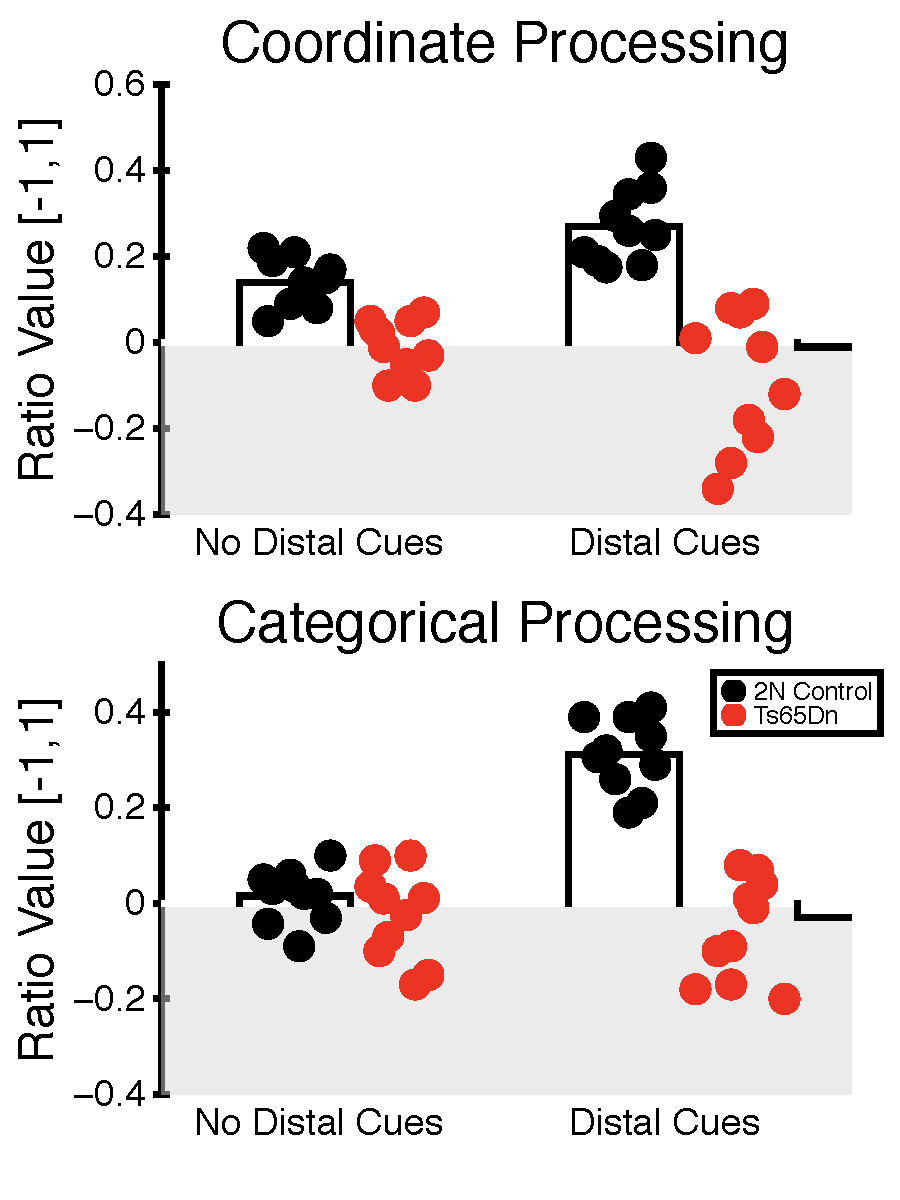
\includegraphics[scale=1]{CategoricalCoordinate.pdf}
\caption{Top. Metric/Coordinate processing performance in the presence and absence of extra-maze, distal cues.}
\label{fig:MetricTopological}
\end{figure}

textbf{Topological/Categorical Processing}

For detection of a topological change, Ts65Dn mice showed significant impairments relative to 2N control mice. There was a main effect for groups for the clear box (F(1,18)=78.52,p<5.55e-8) but not for the red box (F(1,18)=1.489,p=.238).

\begin{figure}[h!]
\centering
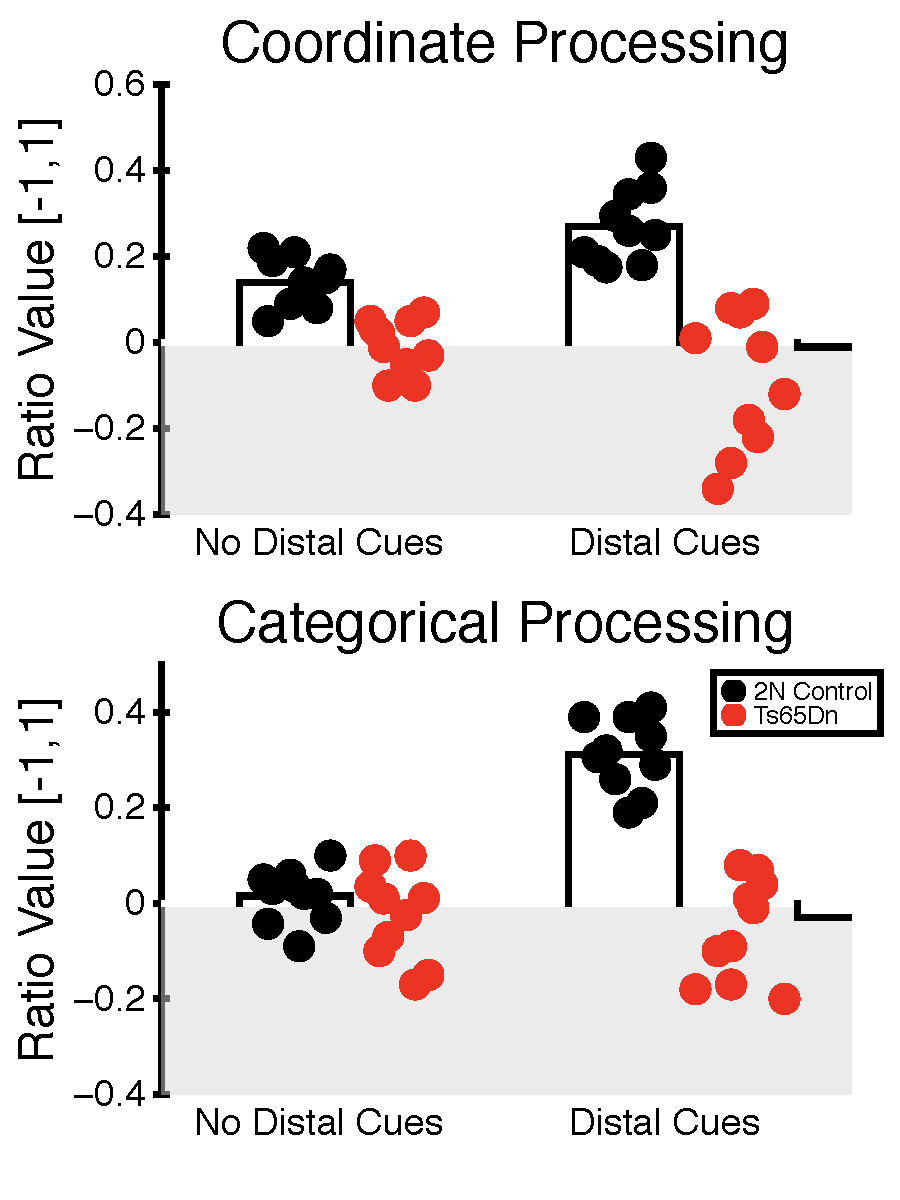
\includegraphics[scale=1]{CategoricalCoordinate.pdf}
\caption{Bottom. Topological/Categorical processing performance in the presence and absence of extra-maze, distal cues.}
\label{fig:MetricTopological}
\end{figure}

textbf(Location Recognition)

For detection of a change int he spatial location of a visual object, Ts65Dn mice showed significant impairments relative to 2N control mice. There was a main effect for groups for the clear box (F(1,18)=36.39,p<1.05e-5) as well as in the red box (F(1,18)=62.0,p=3.07e-7).

\begin{figure}[h!]
\centering
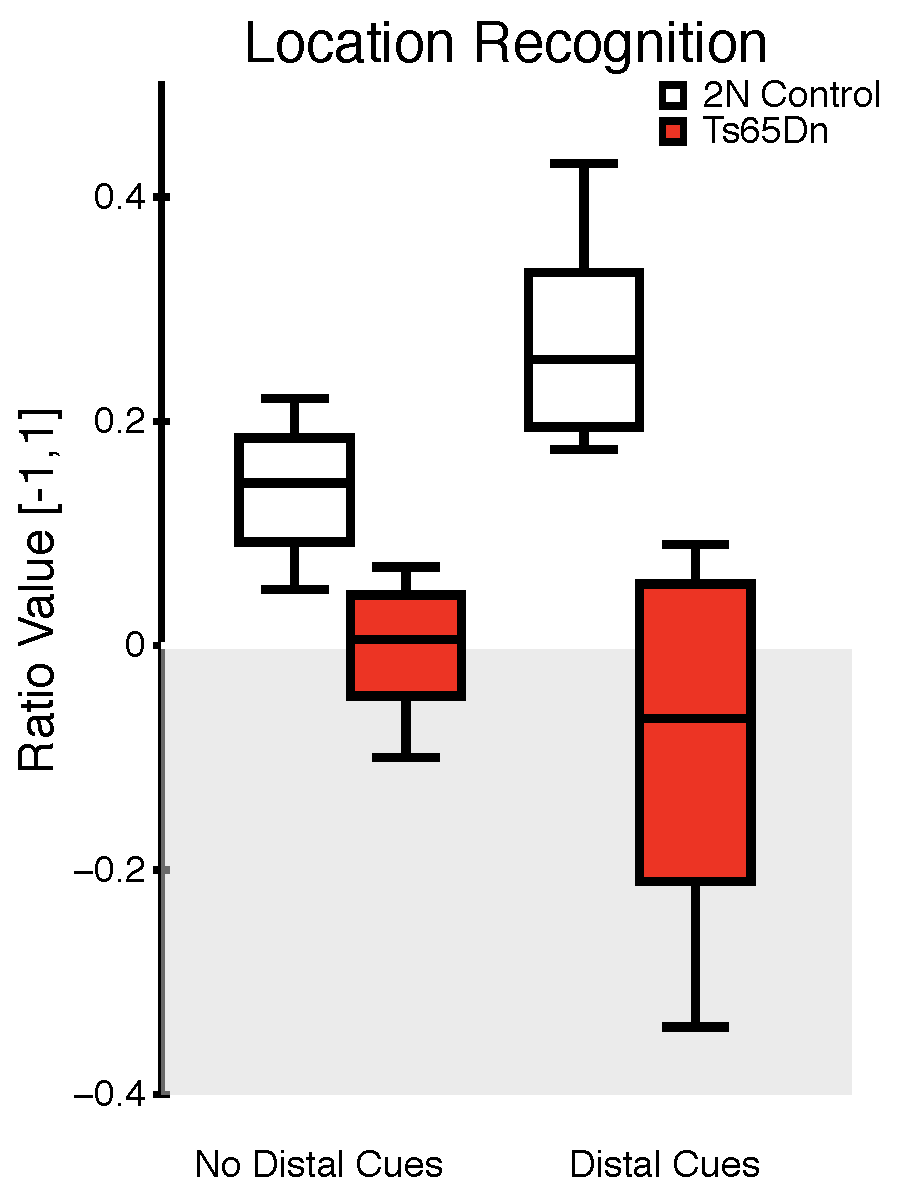
\includegraphics[scale=1]{LocRec.pdf}
\caption{Spatial Location recognition performance in the presence and absence of extra-maze, distal cues}
\label{fig:LocationRecognition}
\end{figure}

\subsection{Temporal Attribute}

textbf{Temporal Ordering for Visual Objects}

For temporal ordering, Ts65Dn mice did not show significant impairments relative to 2N control mice. There was a main effect for groups for the clear box (F(1,18)=68.24,p<1.55e-7) but not for the red box (F(1,18)=2.267,p=.149). These data suggest that the presence of spatial cues, but not temporal ordering resulted in deficits in the clear box.

\begin{figure}[h!]
\centering
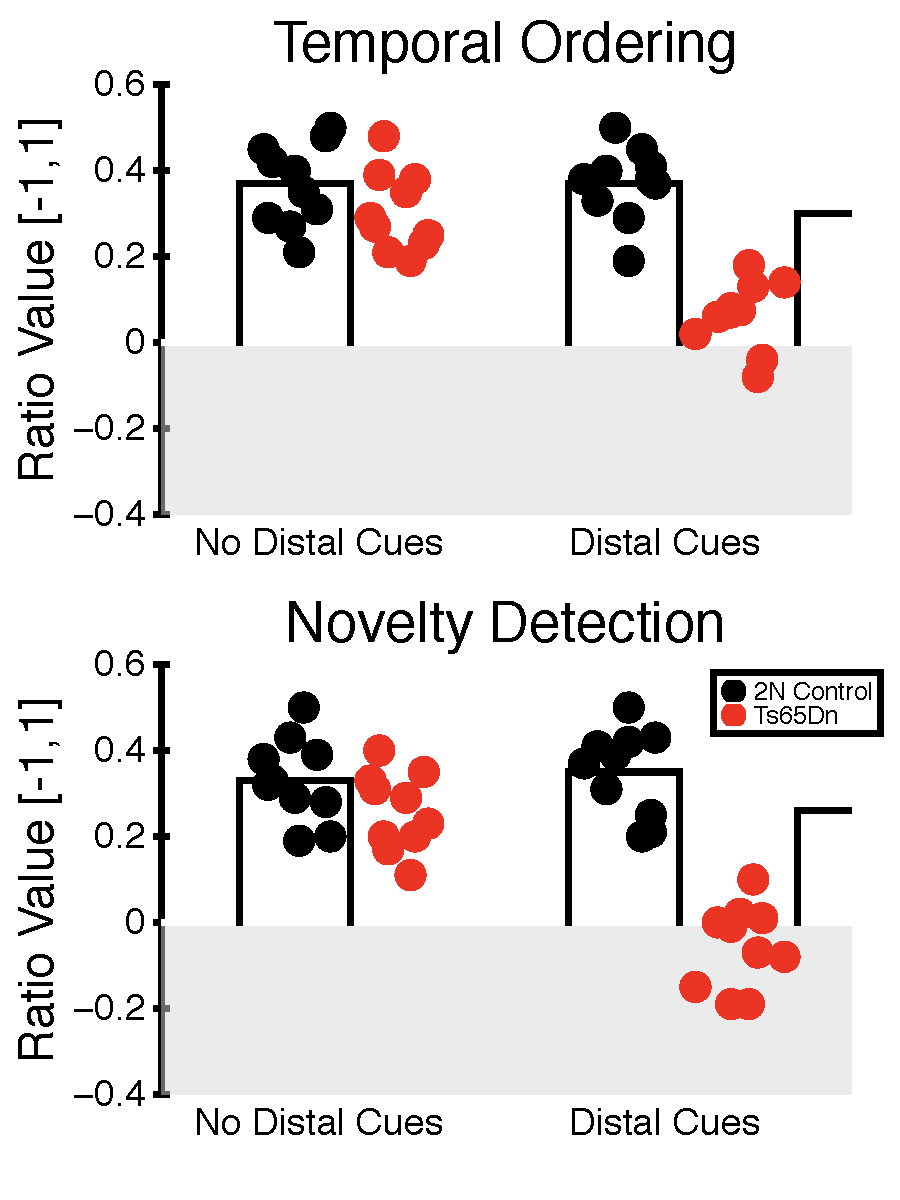
\includegraphics[scale=1]{TempOrder.pdf}
\caption{Top. Temporal ordering for visual objects in the presence and absence of extra-maze, distal cues}
\label{fig:TemporalOrder}
\end{figure}

textbf{Temporal Order Control Task: Novelty Detection for Visual Objects}

For the novelty detection task run as a control for temporal ordering, Ts65Dn mice did not show significant impairments relative to 2N control mice. There was a main effect for groups for the clear box (F(1,18)=82.78,p<3.74e-8) but not for the red box (F(1,18)=2.909,p=.105). These data suggest that the presence of spatial cues, but not temporal ordering or novelty detection resulted in deficits in the clear box.

\begin{figure}[h!]
\centering
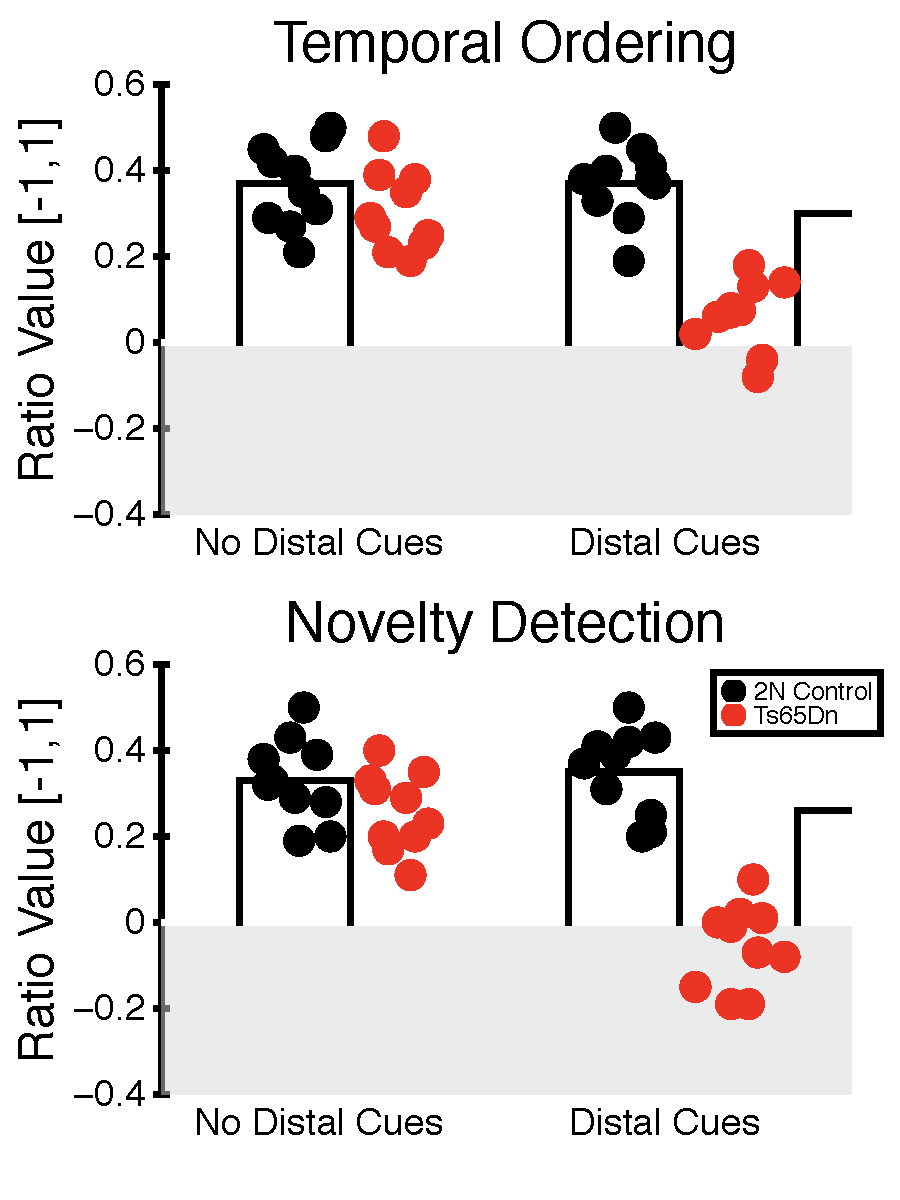
\includegraphics[scale=1]{TempOrder.pdf}
\caption{Bottom. Visual object novelty detection control task in the presence and absence of extra-maze, distal cues}
\label{fig:TemporalOrder}
\end{figure}

\subsection{Sensory/Perceptual Attribute}

textbf{Feature Ambiguity}

For detection of configural feature ambiguity, Ts65Dn mice did not show significant impairments relative to 2N control mice. There was a main effect for groups for the clear box (F(1,18)=34.13,p<1.56e-5) but not for the red box (F(1,18)=.021,p=.984). These data suggest that the presence of spatial cues, but not configural feature ambiguity resulted in deficits in the clear box.

\begin{figure}[h!]
\centering
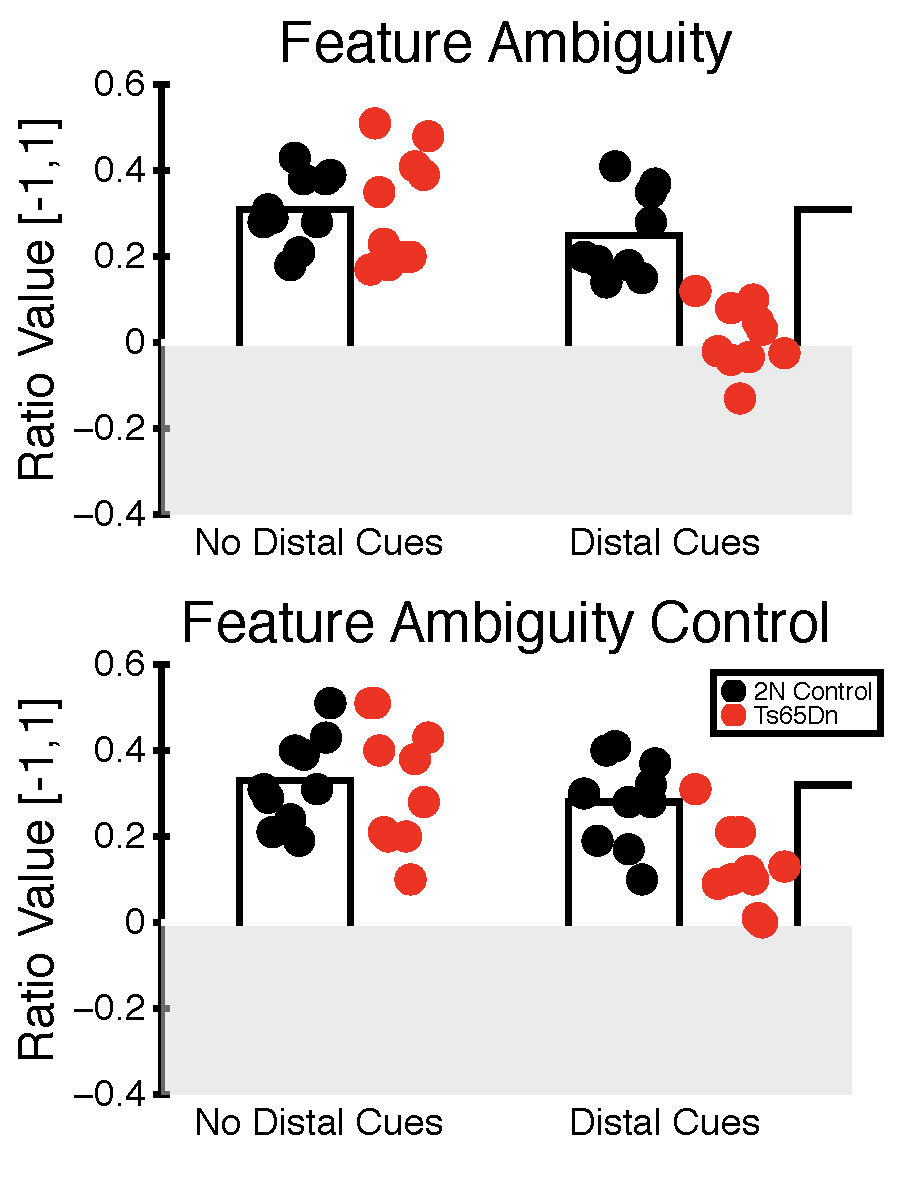
\includegraphics[scale=1]{Ambiguous.pdf}
\caption{Top. Configural feature ambiguity test in the presence and absence of extra-maze, distal cues}
\label{fig:Ambiguity}
\end{figure}

textbf{Feature Ambiguity Control Task: Novelty Detection for Configural Object}

For detection of configural feature novelty, Ts65Dn mice showed significant impairments relative to 2N control mice. There was a main effect for groups for the clear box (F(1,18)=12.27,p=.00254) but not for the red box (F(1,18)=.012,p=.916). These data suggest that the presence of spatial cues, but not configural feature novelty detection ordering resulted in deficits in the clear box.

\begin{figure}[h!]
\centering
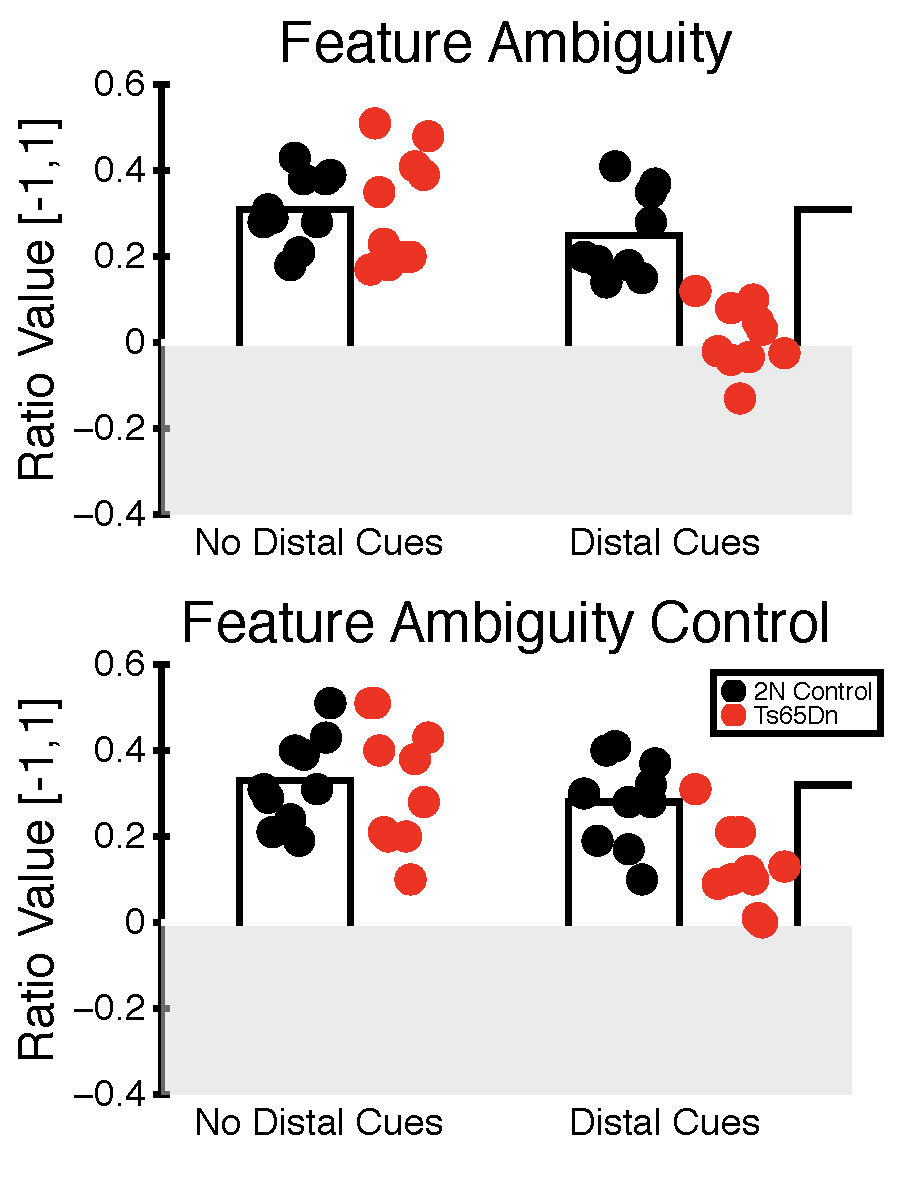
\includegraphics[scale=1]{Ambiguous.pdf}
\caption{Bottom. Novel Configural ambiguity control test in the presence and absence of extra-maze, distal cues}
\label{fig:Ambiguity}
\end{figure}

textbf{Object Recognition}

textbf{Short (1 hr) Delay}

For object recognition memory at 1 hour, Ts65Dn mice did not show significant impairments relative to 2N control mice. There was a main effect for groups for the clear box (F(1,18)=29.51,p<3.68e-5) but not for the red box (F(1,18)=.908,p=.353). These data suggest that the presence of spatial cues, but not object recognition resulted in deficits in the clear box.

\begin{figure}[h!]
\centering
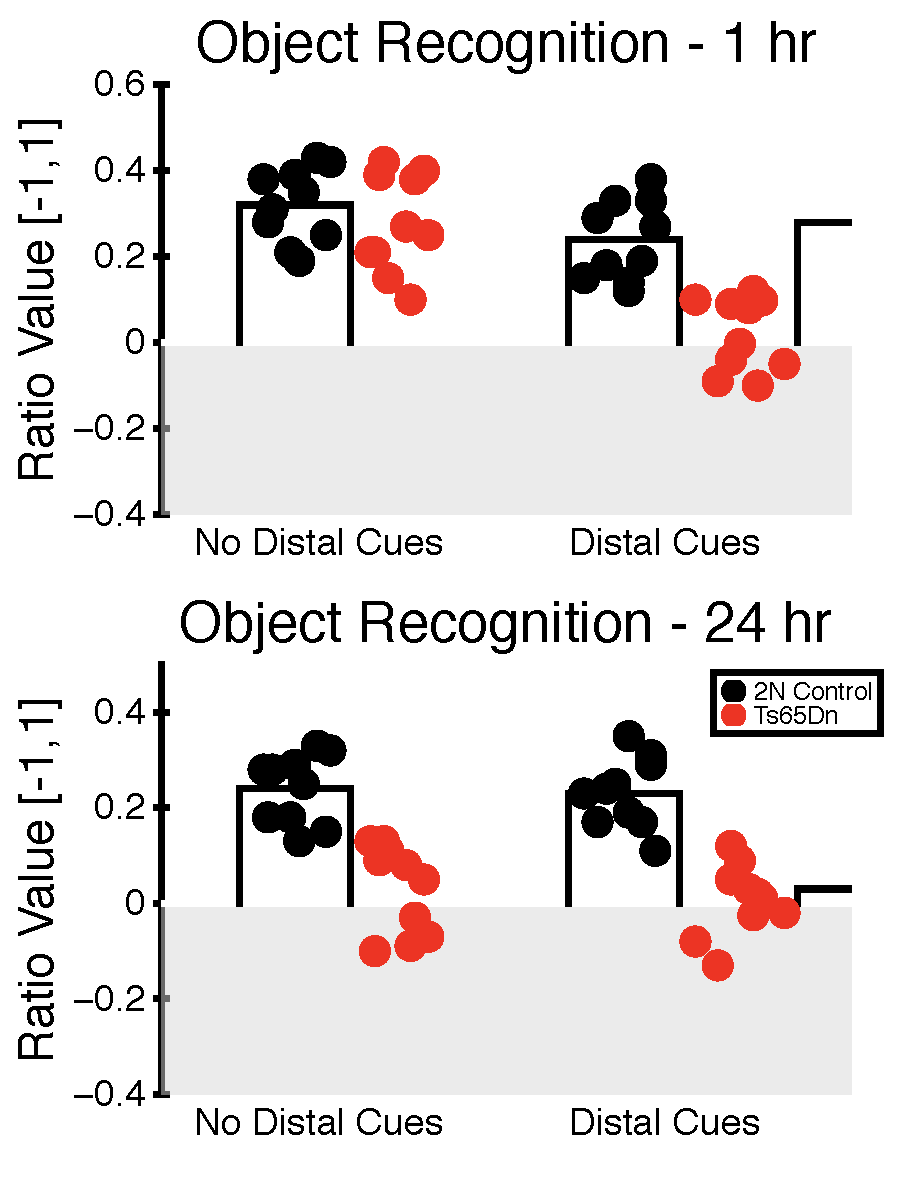
\includegraphics[scale=1]{ObjectRec.pdf}
\caption{Top. Visual object recognition task at 1 hour delay the presence and absence of extra-maze, distal cues}
\label{fig:ObjectRecognition}
\end{figure}

textbf{Long (24 hr) Delay}

For object recognition memory at 24 hours, Ts65Dn mice did not show significant impairments relative to 2N control mice. There was a main effect for groups for the clear box (F(1,18)=46.23,p<2.29e-6) as well as for the red box (F(1,18)=31.36,p=2.58e-5). These data suggest that the presence of spatial cues, but not object recognition resulted in deficits in the clear box.

\begin{figure}[h!]
\centering
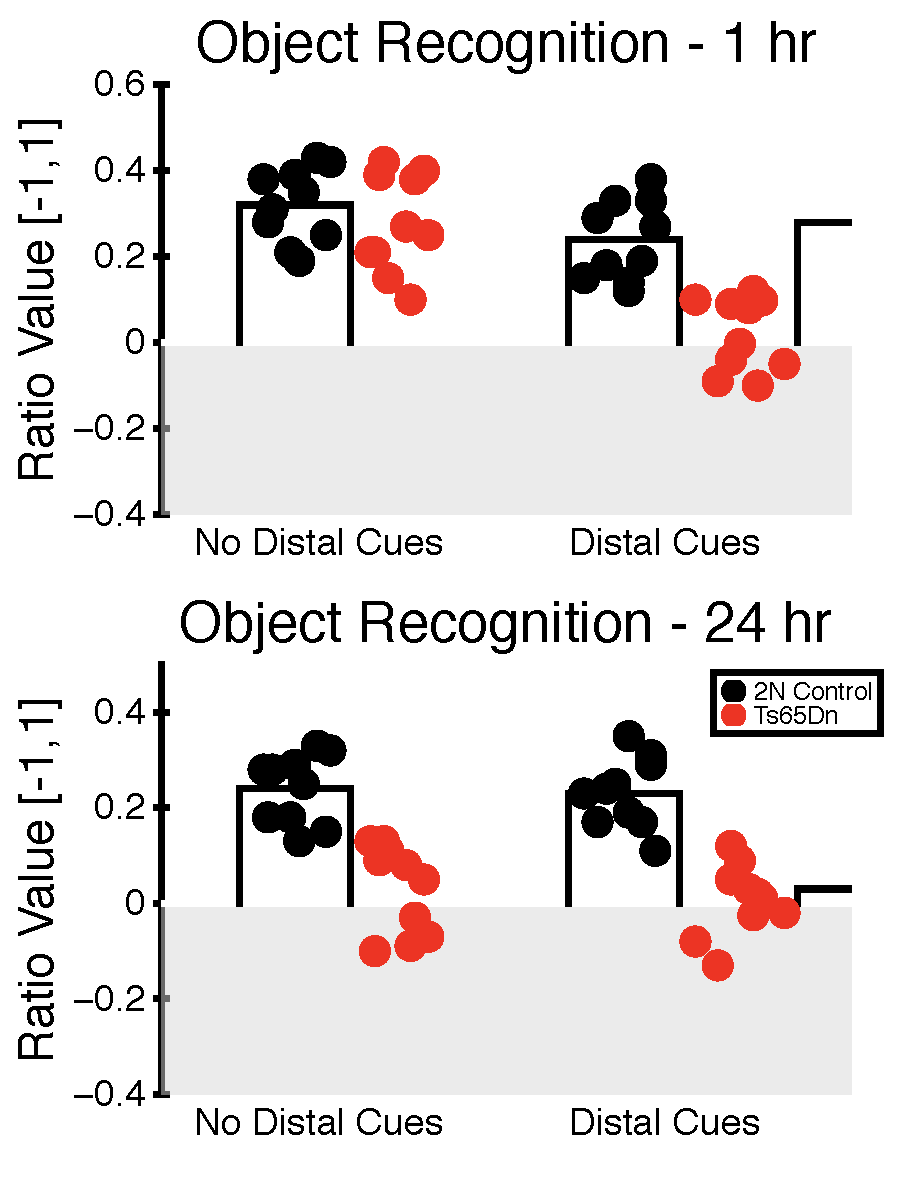
\includegraphics[scale=1]{ObjectRec.pdf}
\caption{Bottom. Visual object recognition task at 24 hour delay the presence and absence of extra-maze, distal cues}
\label{fig:ObjectRecognition}
\end{figure}

\subsection{Rule Based Memory System/Executive Function}

textbf{Spontaneous Alternation}

For spontaneous alternation, Ts65Dn mice showed fewer alternations than 2N control mice (F(1,18)=23.85,p=.00012).

\begin{figure}[h!]
\centering
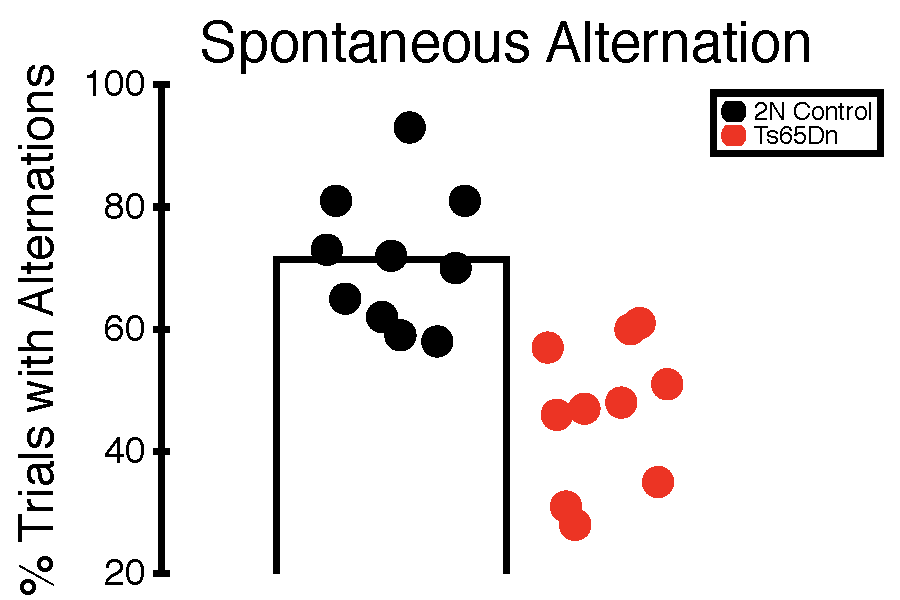
\includegraphics[scale=1]{SpontaneousAlternation.pdf}
\caption{Spontaneous/Delayed Alternation performance}
\label{fig:SpontaneousAlternation}
\end{figure}

textbf{Response Learning}

For the learning of a turn response, Ts65Dn mice took significantly longer to learn the rule than 2N control mice. There was a main effect for groups (F(1,76)=30.24,p=4.92e-7), a main effect for block of trials (F(1,76)=502.86,p<2e-16). There was also an interaction among group and block (F(1,76)=7.82,p=.00654). This interaction was the result of the Ts65Dn mice taking longer to learn the rule. For the final block of 20 trials, there were no differences in performance for Ts65Dn and 2N control mice.

\begin{figure}[h!]
\centering
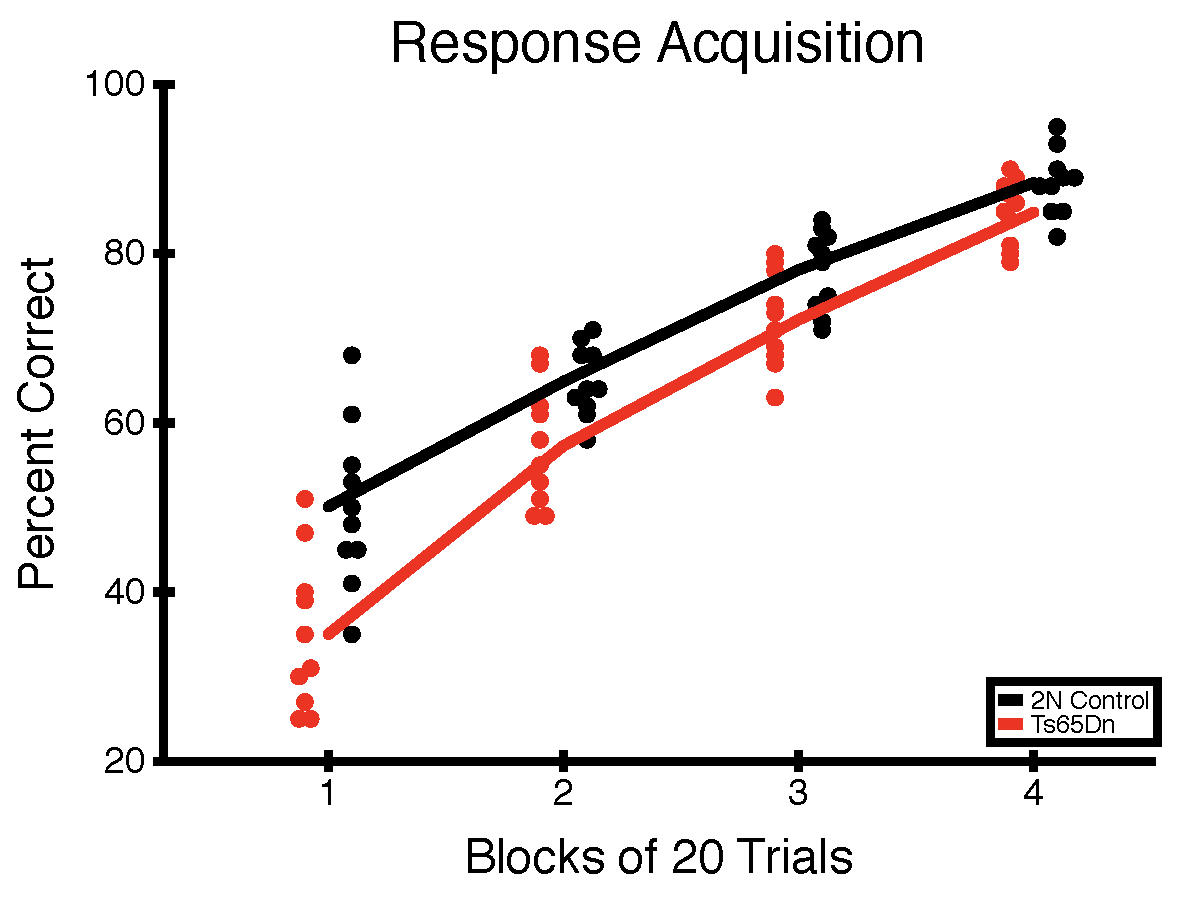
\includegraphics[scale=1]{ResponseAcquisition.pdf}
\caption{Response rule acquisition}
\label{fig:ResponseAcquisition}
\end{figure}

textbf{Rule Reversal Learning}

\begin{figure}[h!]
\centering
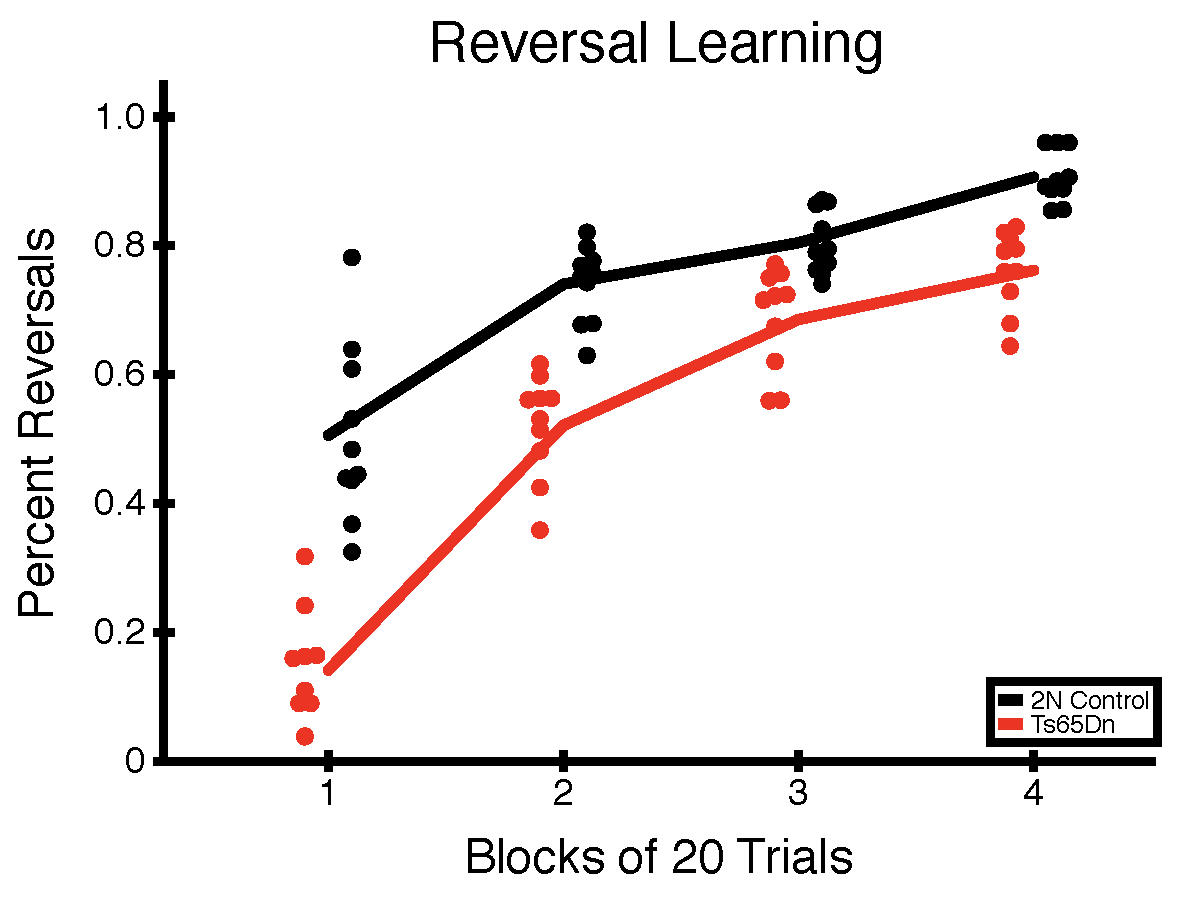
\includegraphics[scale=1]{Reversal_RAW.pdf}
\caption{Response rule reversal raw data converted to cumulative response}
\label{fig:ReversalRAW}
\end{figure}

For reversal learning, Ts65Dn mice showed significant impairments relative to 2N control mice. There was a main effect for groups for the trial at which the mice changed preference from old rule to new rule (changepoint; F(1,18)=21.43,p=.000208). For the first 20 trials of reversal learning, Ts65Dn mice showed a greater number of perseverative errors (F(1,18)=11.98,p=.00278). For trials 21-40, there was no difference between Ts65Dn mice and 2N control mice for regressive errors (F(1,18)=.287,p=.599).

\begin{figure}[h!]
\centering
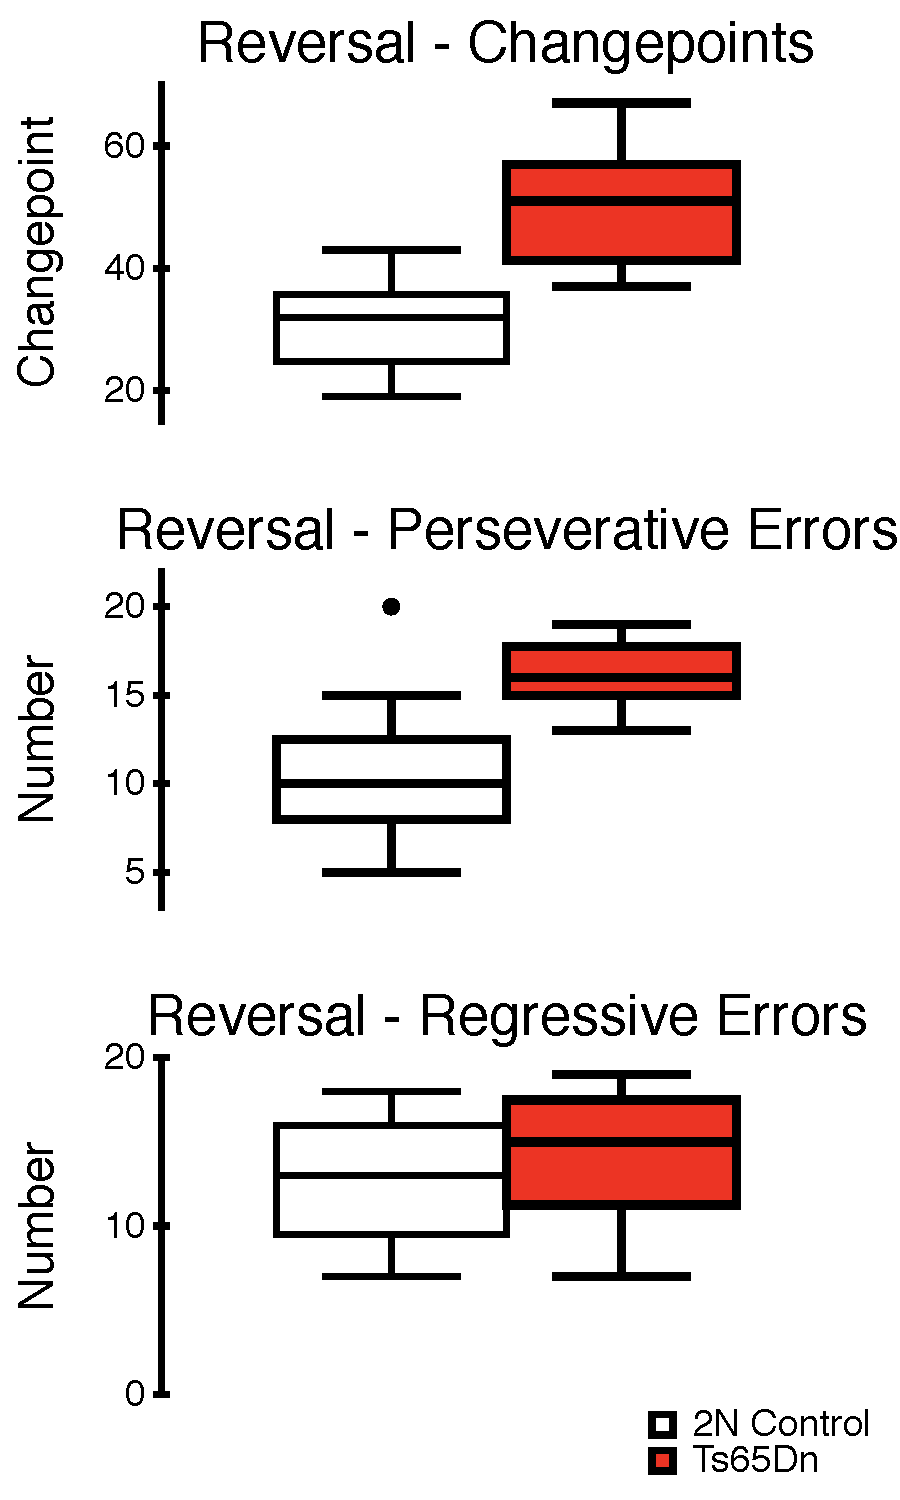
\includegraphics[scale=1]{Reversal_Factors.pdf}
\caption{Top. Changepoint, or trial at which each mouse learned to reverse the rule. Middle. Number of perseverative errors in trial 1-20 trials. Bottom. Number of Regressive erros in trials 20-40}
\label{fig:ReversalFactors}
\end{figure}

\subsection{Motor Function}

textbf{Capellini Handling}

For the capellini task, Ts65Dn mice showed significant impairments relative to 2N control mice. There was a main effect for latency, with Ts65Dn mice taking longer to eat the pasta on average (F(1,18)=14.74,p=.0012). Ts65Dn mice also made a greater number of pasta handling errors (F(1,18)=92.68,p=1.6e-8)

\begin{figure}[h!]
\centering
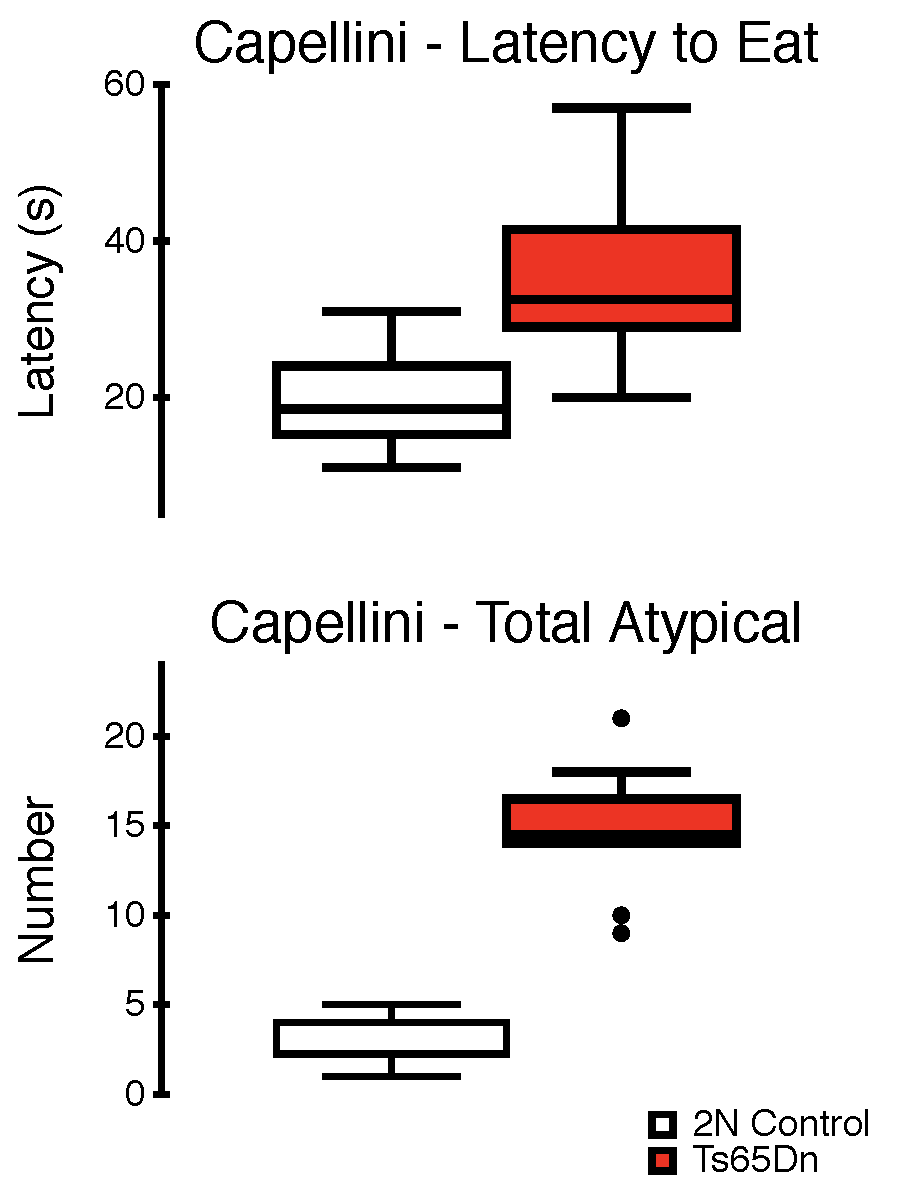
\includegraphics[scale=1]{Capellini_Latency.pdf}
\caption{Top. Latency to consume capellini. Bottom. Total number of atypical behaviors}
\label{fig:CapelliniLatency}
\end{figure}

For type of errors in the capellini handling task, Ts65Dn mice showed significant impairments relative to 2N control mice. There was a main effect for groups for the number of times the paws came together (F(1,18)=42.34,p=4.06e-6), for the number of times the mouse lost contact with the pasta (F(1,18)=20.35,p=.00027)and the number of times the mouse pulled the pasta with their mouth rather than using the hands to move it (F(1,18)=21.46,p=.000207).

\begin{figure}[h!]
\centering
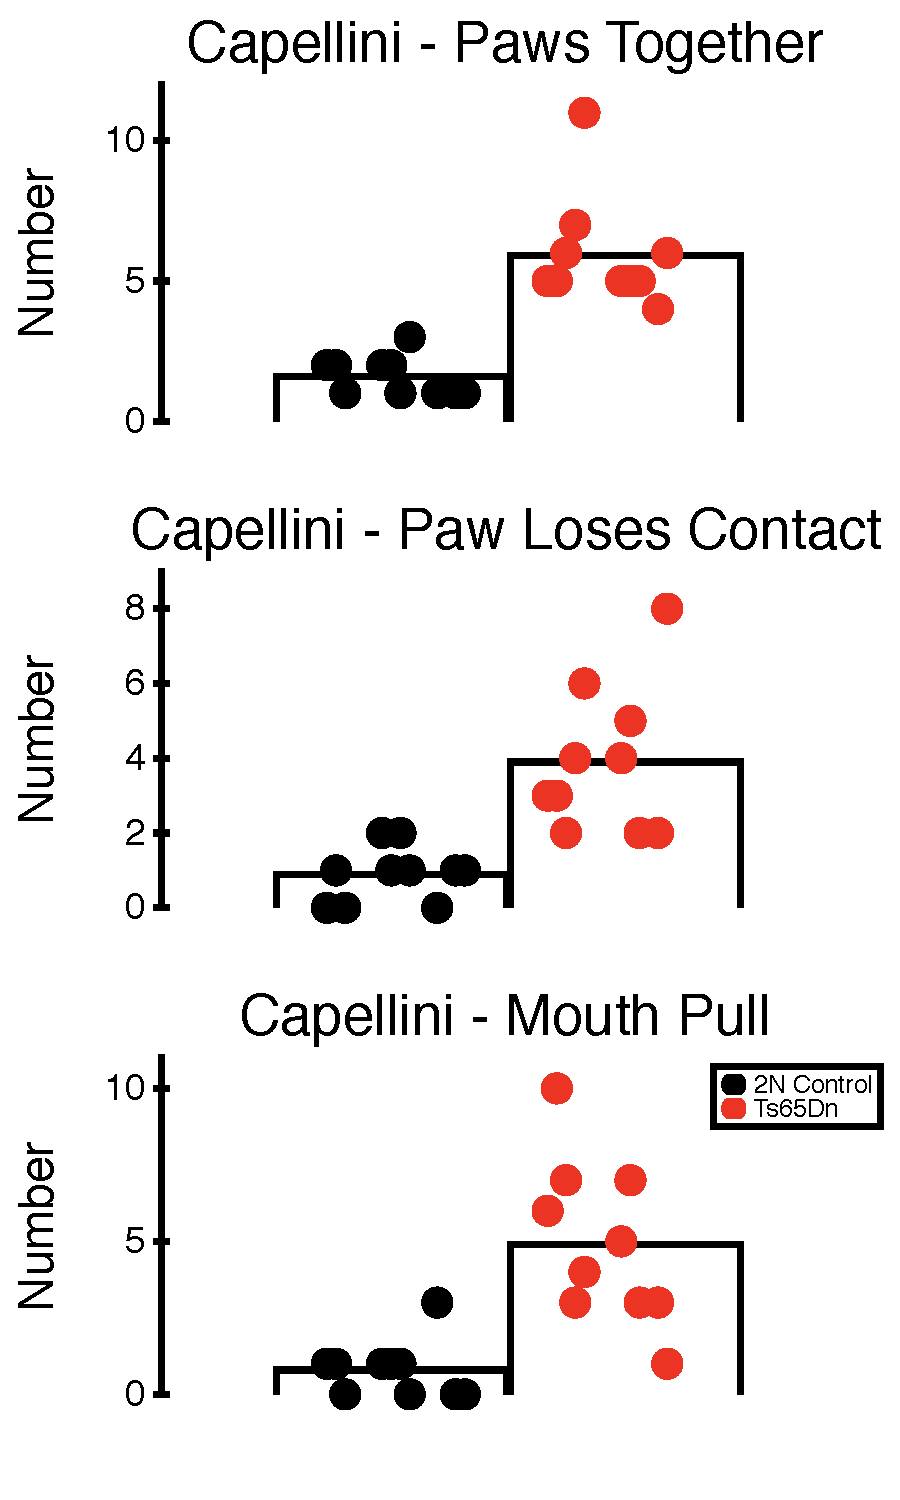
\includegraphics[scale=1]{Capellini_Errors.pdf}
\caption{Atypical Behaviors. Top. Number of times mouse paws came together. Middle. Number of times mouse lost contact with capellini with one paw. Bottom. Number of times mouse pulled capellini with mouth rather than paw}
\label{fig:CapelliniErrors}
\end{figure}

textbf{Parallel Rung Walking}

For the parallel rung walking task, Ts65Dn mice showed significant impairments relative to 2N control mice. There was a main effect for the number of foot slips in a 1 minute session (F(1,18)=27,32,p=5.7e-5).  When adjusted for number of steps, Ts65Dn mice still showed a greater number of foot slip errors (F(1,18)=11.70,p=.00305)

\begin{figure}[h!]
\centering
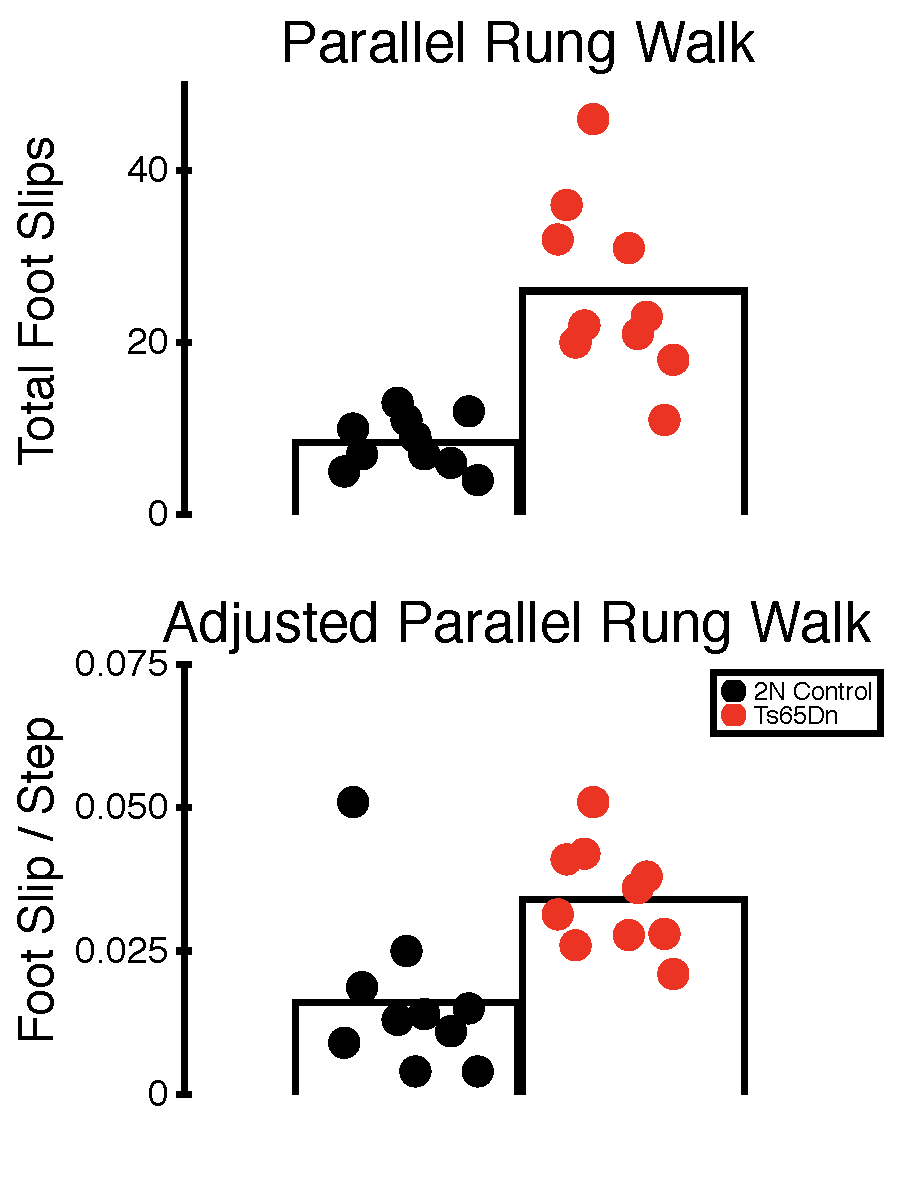
\includegraphics[scale=1]{ParallelRung.pdf}
\caption{Top. Raw number of foot slips in a 1 minute period of free exploration. Bottom. Number of foot slips scaled by the total number of steps}
\label{fig:ParallelRung}
\end{figure}

\subsection{Adaptive Function/Quality of Life}

textbf{Nesting Behaviors}

Ts65Dn mice showed significant impairments relative to 2N control mice for nesting measures. Ts65Dn mice took longer to make contact with the nesting material (F(1,18)=152.9,p=3.1e-10), for the time it took for them to dig in the media (measured from time of first contact) (F(1,18)=318.6,p=6.79e-13), and the time it took from starting to dig to finish the nest (F(1,18)=94.3,p=1.4e-8).

\begin{figure}[h!]
\centering
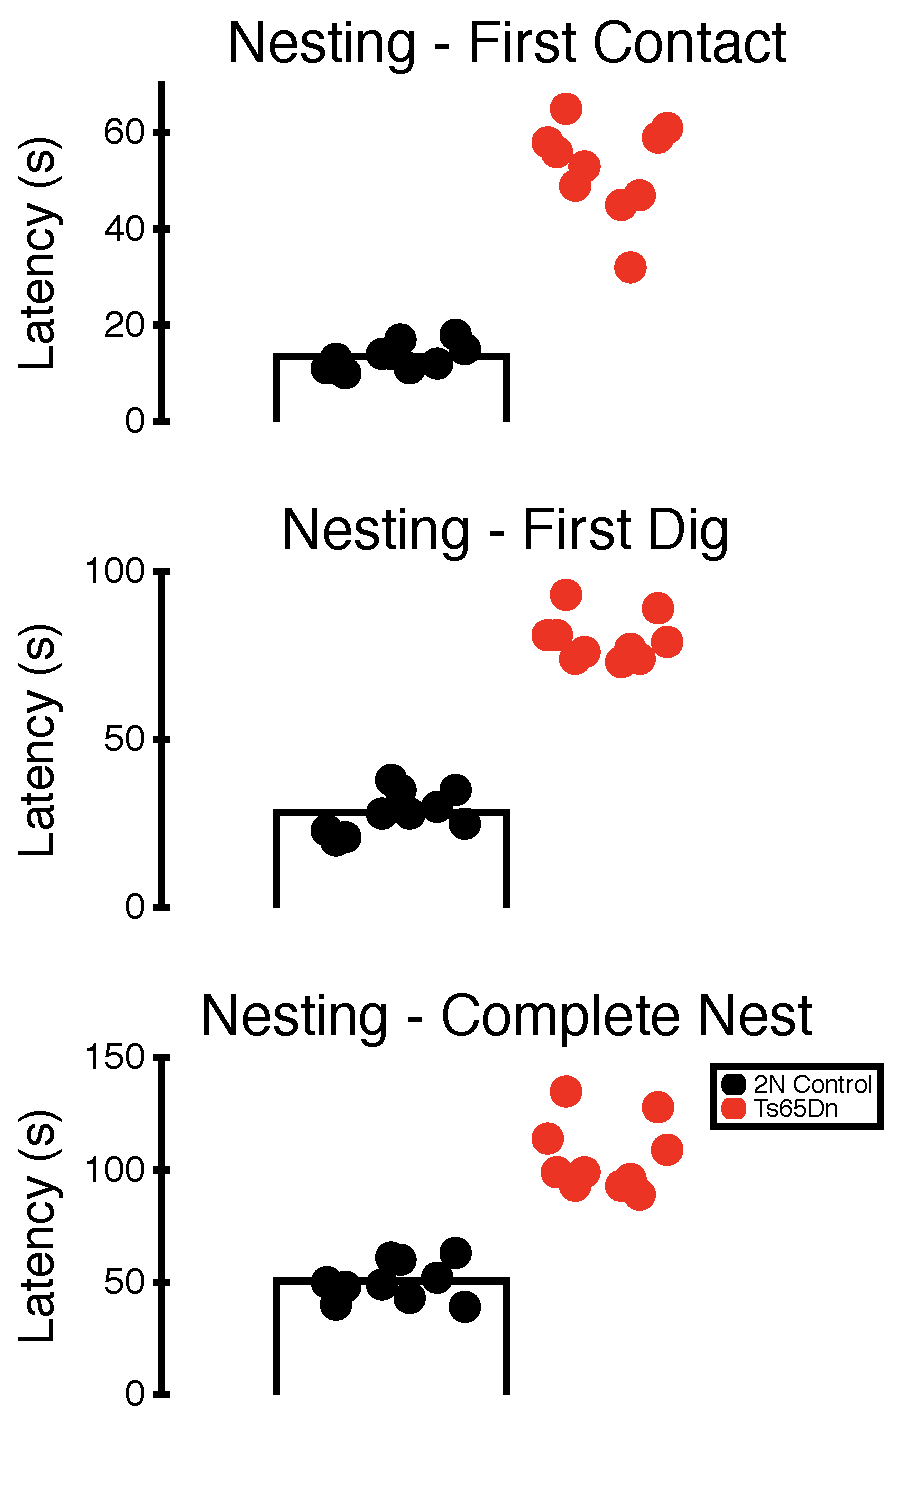
\includegraphics[scale=1]{Nesting.pdf}
\caption{Nesting Behaviors. Top. Latency to contact nesting material. Middle. Latency to first dig in nesting material. Bottom. Latency to complete nest}
\label{fig:Nesting}
\end{figure}

textbf{Neophobia}

Ts65Dn mice showed significant impairments relative to 2N control mice for neophobia. Ts65Dn mice took longer to eat a novel food in a familiar environment(F(1,18)=19.59,p=.000326), took longer to eat a familiar food in a novel environment(F(1,18)=40.87,p=5.09e-6), and took longer to eat a novel food in a novel environment(F(1,18)=83.74,p=3.44e-8).

\begin{figure}[h!]
\centering
\includegraphics[scale=1]{Neophobia.pdf}
\caption{Neophagia Behaviors. Top. Latency to start to consume novel food in a familiar environemnt. Middle. Latency to start to consume familiar food in a novel environemnt. Bottom. Latency to start to consume a novel food in a novel environment}
\label{fig:Neophobia}
\end{figure}

\subsection{Grouping Tasks by Domain: Principal Component Analysis}

To determine if there were a general structure to the tasks being used in the mouse ACTB, a principal component analysis was performed. This PCA analysis identified 2 main clusters, with one axis accounting for 57.76\% of the variance. This clustered the tasks into groups with all the spatiotemporal tasks and spontaneous alternation in one group, and the executive, motor, and adaptive function tasks comprising a second cluster. When this clustering was used to sort the mice into groups, the principal axis was sufficient to sort the mice into appropriate Ts65Dn and 2N control groups.

\begin{figure}[h!]
\centering
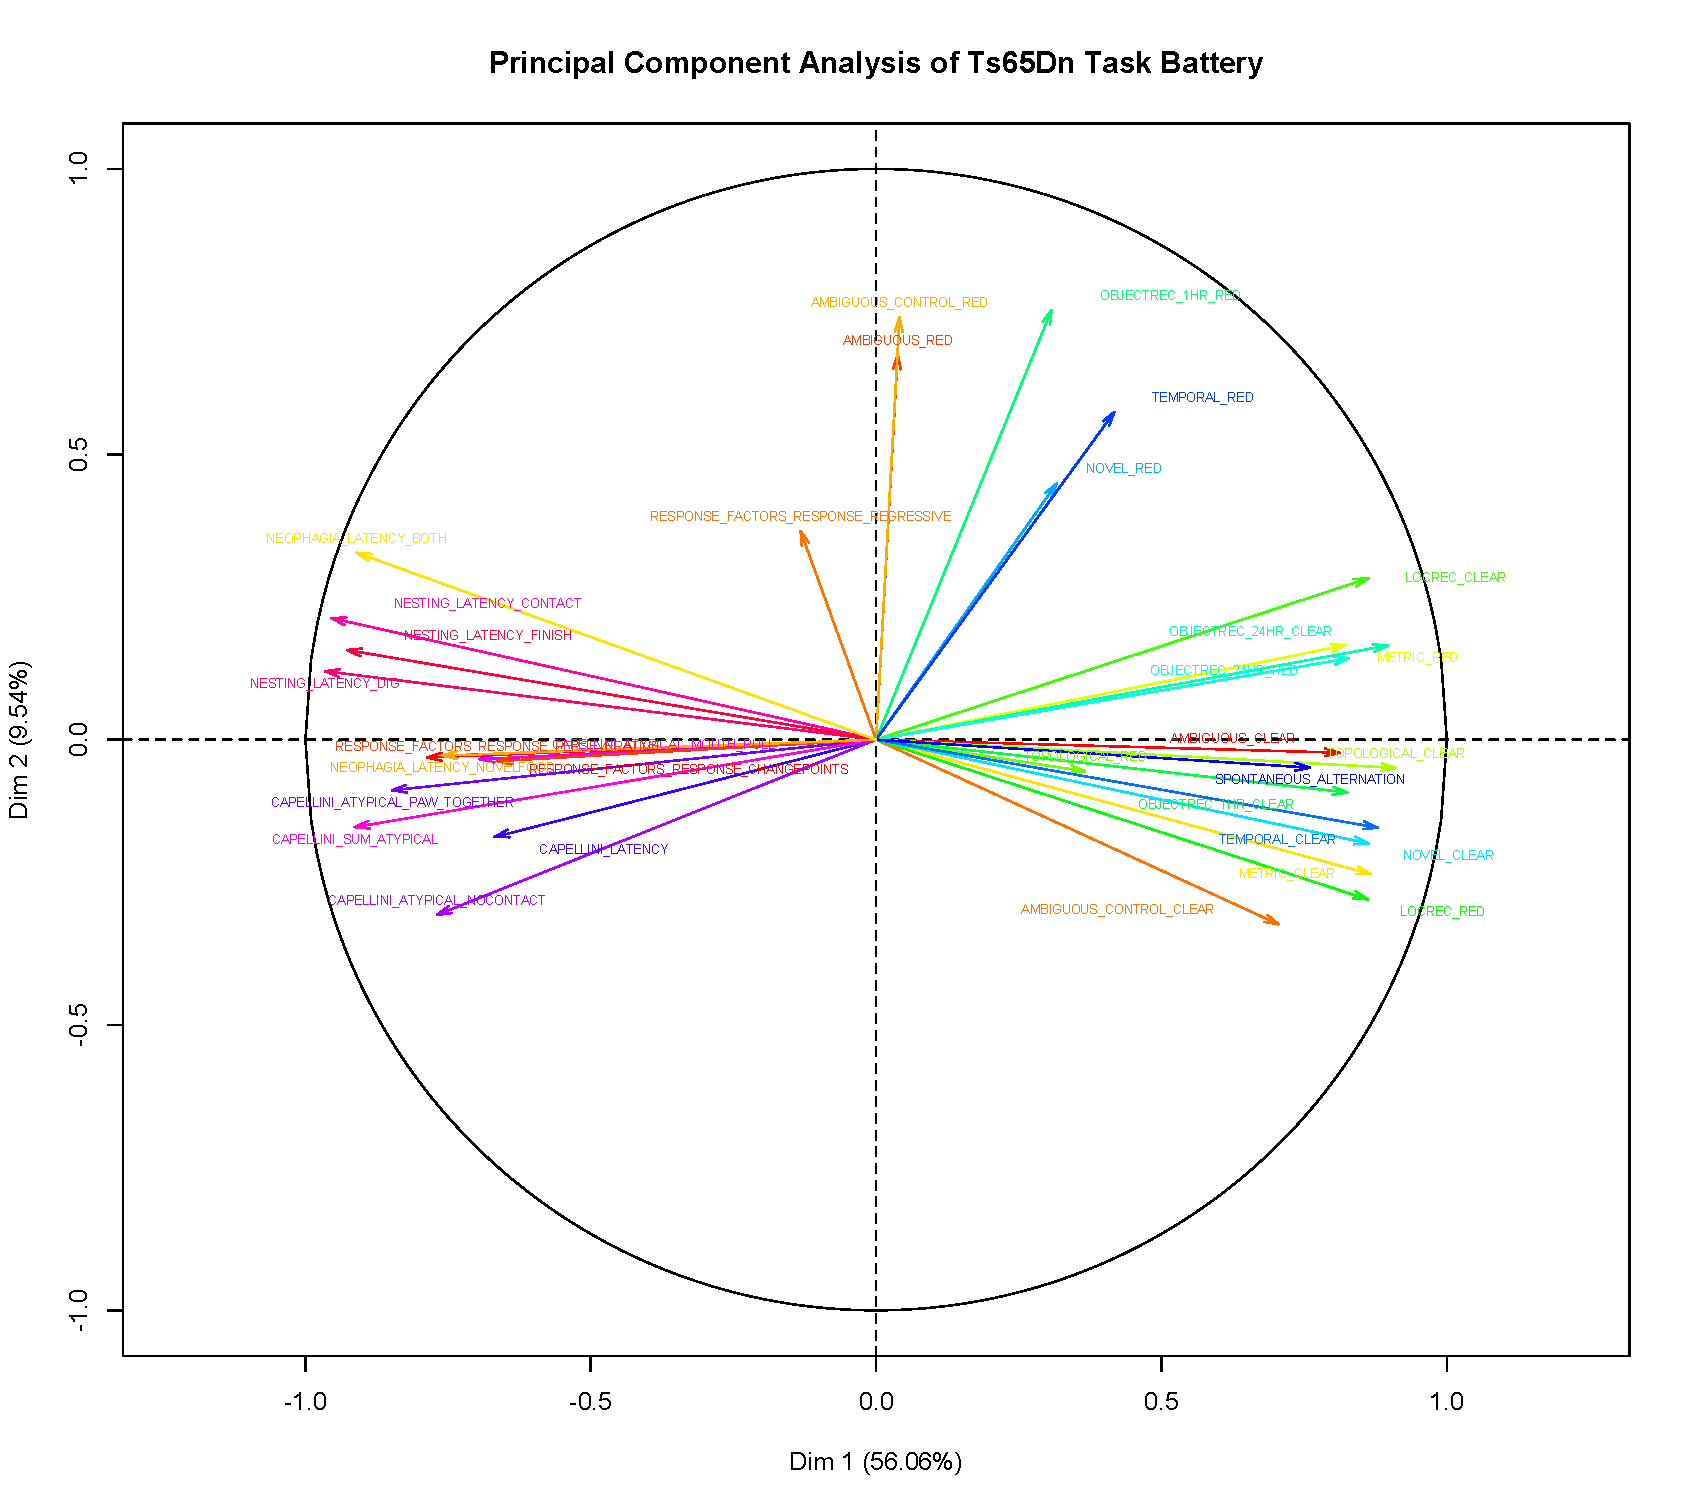
\includegraphics[scale=1]{PCA_Tasks.pdf}
\caption{Principal Component Analysis focusing on behavioral paradigms. Two major components emerge, accounting for 57.76% of the variance. These components seem to be behavioral tasks dependent upon MTL structures clustering together and executive+motor+adaptive function components clustering together}
\label{fig:PCA Tasks}
\end{figure}

\begin{figure}[h!]
\centering
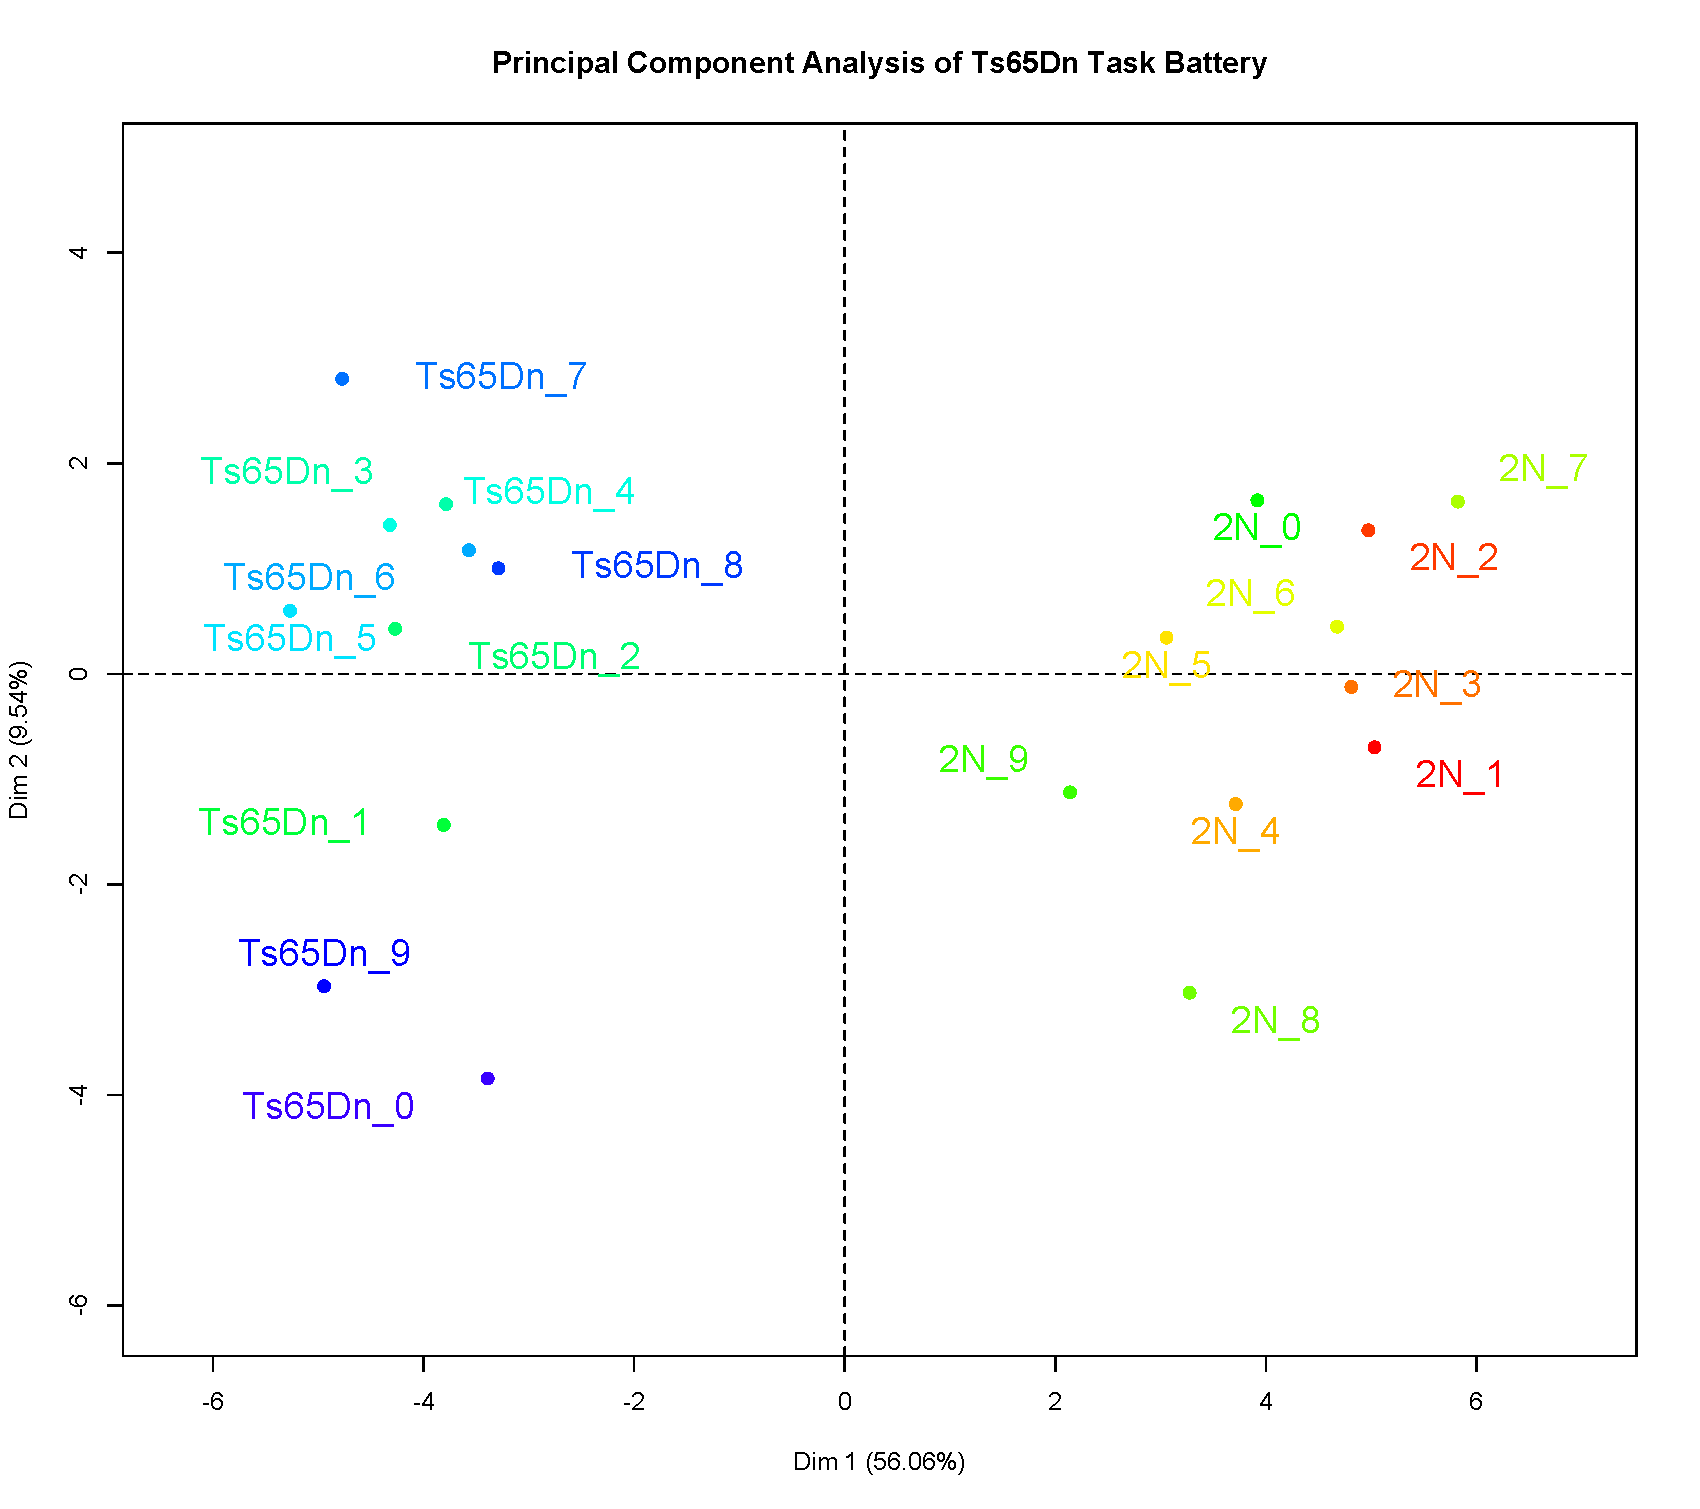
\includegraphics[scale=1]{PCA_Sorting.pdf}
\caption{Principal Component Analysis focusing on behavioral paradigms. Using the components extracted above, all mice were correctly sorted into groups using the primary component. The secondary component accounting for slightly over 9% of the variance failed to sort the groups effectively}
\label{fig:PCA Groups}
\end{figure}

\section{Discussion}
\subsection{General Discussion}

Mouse ACTB tests same brain regions and cognitive domains as the ACTB designed for use in Down Syndrome subjects

Ts65Dn mice show spatiotemporal, motor, executive, and adaptive functioning deficits

Ts65Dn Mouse behaviorally phenocopies human subjects with Down Syndrome when given appropriate tasks

Mouse version of ACTB can be used to more specifically assess contributions of different brain regions for intellectual disabilities observed in Down Syndrome

Mouse ACTB may serve as a Down Syndrome-specific outcome measure for tests of novel therapeutics

Potentially use this mouse ACTB to define prodromal states in Ts65Dn mouse for putative Alzheimer's Disease-like phenotypes or progression

List touchscreen tasks from Tim Bussey that model essentially the same thing as a great direction/alternative to mine.

\subsection{Strengths of the mouse ACTB}

None of these tasks require specialized equipment or expertise and are thus accessible to most disease researchers

Behavioral paradigms carefully/specifically optimized to mouse models

Contributions of spatial and nonspatial attributes dissociated within each task

All but 2 tasks were performed in 2 days or less \(high throughput\)

No aversive components to tasks \(i.e., no negative reinforcement or aversive stimulus used to motivate\)

Can specifically dissect contribution of basic cognitive processes and  brain areas to performance

Previous work has demonstrated these tasks can be repeated for use in longitudinal studies

\subsection{Weaknesses of the mouse ACTB}

We are unable to evaluate receptive vs. expressive language in mouse models

Ts65Dn mouse model not necessarily best model for Down Syndrome genetics

\subsection{Future Directions}

Eugene Yu's 16/17/10 mouse model \(best genetic mouse model of Down Syndrome\)

Single gene studies \(i.e., App, Dyrk1, pep19/pcp4, etc. triploid mice\)

Cell specific genetic models

Ultrasonic vocalization studies for linguistic analog

Tasks to test affective attributes of memory

``I always thought something was fundamentally wrong with the universe'' \citep{adams1995hitchhiker}

\bibliographystyle{plain}
\bibliography{references}
\end{document}
